\newcommand{\dands}{\foreignlanguage{english}{Delay-and-Sum}}
\newcommand{\micname}{MP45DT02}
\newcommand{\boardname}{Terasic DE2-115}

% !TeX spellcheck = russian-aot-ieyo
% Зачем: Определяет класс документа (То, как будет выглядеть документ)
% Примечание: параметр draft помечает строки, вышедшие за границы страницы, прямоугольником, в фильной версии его нужно удалить.
\documentclass[a4paper,14pt,oneside,draft]{extreport}

% Генерит только определенные страницы
%\usepackage[36-41]{pagesel}

% Зачем: Выбор внутренней TeX кодировки.
\usepackage[T2A]{fontenc}

% Зачем: Предоставляет проприетарный Times New Roman.
% ОБНОВЛЕНИЕ: лучше использовать scalable-cyrfonts-tex: меньше проблем с установкой
% Из руководства к PSCyr: "Во избежание проблем пакет PSCyr должен загружаться перед пакета-ми inputenc и babel".
% Примечание: Требует шаманства при установке, инструкция http://plumbum-blog.blogspot.com/2010/06/miktex-28-pscyr-04d.html
% http://blog.harrix.org/?p=444
% надо закомментировать это, чтобы использовать scalable-cyrfonts-tex:
\usepackage{pscyr}

% Зачем: Установка кодировки исходных файлов.
\usepackage[utf8]{inputenc}

% Зачем: Предоставляет свободный Times New Roman.
% Шрифт идёт вместе с пакетом scalable-cyrfonts-tex в Ubuntu/Debian
% раскомментировать, чтобы использовать scalable-cyrfonts-tex:
%\usefont{T2A}{ftm}{m}{sl}

% Зачем: Делает результирующий PDF "searchable and copyable".
\usepackage{cmap}

% Зачем: Чтобы можно было использовать русские буквы в формулах, но в случае использования предупреждать об этом.
\usepackage[warn]{mathtext}

% Зачем: Учет особенностей различных языков.
\usepackage[english, russian]{babel}

% Зачем: Добавляет поддержу дополнительных размеров текста 8pt, 9pt, 10pt, 11pt, 12pt, 14pt, 17pt, and 20pt.
% Почему: Пункт 2.1.1 Требований по оформлению пояснительной записки.
\usepackage{extsizes}

% Зачем: Длинна, пимерно соответвующая 5 символам
% Почему: Требования содержат странное требование про отсупы в 5 символов (для немоноширинного шрифта :| )
\newlength{\fivecharsapprox}
\setlength{\fivecharsapprox}{6ex}


% Зачем: Добавляет отступы для абзацев.
% Почему: Пункт 2.1.3 Требований по оформлению пояснительной записки.
\usepackage{indentfirst}
\setlength{\parindent}{\fivecharsapprox} % Примерно соответсвует 5 символам.


% Зачем: Настраивает отступы от границ страницы.
% Почему: Пункт 2.1.2 Требований по оформлению пояснительной записки.
\usepackage[left=3cm,top=2.0cm,right=1.5cm,bottom=2.7cm]{geometry}


% Зачем: Настраивает межстрочный интервал, для размещения 40 +/- 3 строки текста на странице.
% Почему: Пункт 2.1.1 Требований по оформлению пояснительной записки.
\usepackage[nodisplayskipstretch]{setspace} 
\setstretch{1.1}
%\onehalfspacing

% Зачем: Выбор шрифта по-умолчанию. 
% Почему: Пункт 2.1.1 Требований по оформлению пояснительной записки.
% Примечание: В требованиях не указан, какой именно шрифт использовать. По традиции используем TNR.
\renewcommand{\rmdefault}{ftm} % Times New Roman


% Зачем: Отключает использование изменяемых межсловных пробелов.
% Почему: Так не принято делать в текстах на русском языке.
\frenchspacing


% Зачем: Сброс счетчика сносок для каждой страницы
% Примечание: в "Требованиях по оформлению пояснительной записки" не указано, как нужно делать, но в других БГУИРовских докуметах рекомендуется нумерация отдельная для каждой страницы
\usepackage{perpage}
\MakePerPage{footnote}


% Зачем: Добавляет скобку 1) к номеру сноски
% Почему: Пункты 2.9.2 и 2.9.1 Требований по оформлению пояснительной записки.
\makeatletter 
\def\@makefnmark{\hbox{\@textsuperscript{\normalfont\@thefnmark)}}}
\makeatother


% Зачем: Расположение сносок внизу страницы
% Почему: Пункт 2.9.2 Требований по оформлению пояснительной записки.
\usepackage[bottom]{footmisc}


% Зачем: Переопределяем стандартную нумерацию, т.к. в отчете будут только section и т.д. в терминологии TeX
\makeatletter
\renewcommand{\thesection}{\arabic{section}}
\makeatother


% Зачем: Пункты (в терминологии требований) в терминологии TeX subsubsection должны нумероваться
% Почему: Пункт 2.2.3 Требований по оформлению пояснительной записки.
\setcounter{secnumdepth}{3}


% Зачем: Настраивает отступ между таблицей с содержанимем и словом СОДЕРЖАНИЕ
% Почему: Пункт 2.2.7 Требований по оформлению пояснительной записки.
\usepackage{tocloft}
\setlength{\cftbeforetoctitleskip}{-1em}
\setlength{\cftaftertoctitleskip}{1em}


% Зачем: Определяет отступы слева для записей в таблице содержания.
% Почему: Пункт 2.2.7 Требований по оформлению пояснительной записки.
\makeatletter
\renewcommand{\l@section}{\@dottedtocline{1}{0.5em}{1.2em}}
\renewcommand{\l@subsection}{\@dottedtocline{2}{1.7em}{2.0em}}
\makeatother


% Зачем: Работа с колонтитулами
\usepackage{fancyhdr} % пакет для установки колонтитулов
\pagestyle{fancy} % смена стиля оформления страниц


% Зачем: Нумерация страниц располагается справа снизу страницы
% Почему: Пункт 2.2.8 Требований по оформлению пояснительной записки.
\fancyhf{} % очистка текущих значений
\fancyfoot[R]{\thepage} % установка верхнего колонтитула
\renewcommand{\footrulewidth}{0pt} % убрать разделительную линию внизу страницы
\renewcommand{\headrulewidth}{0pt} % убрать разделительную линию вверху страницы
\fancypagestyle{plain}{ 
    \fancyhf{}
    \rfoot{\thepage}}


% Зачем: Задает стиль заголовков раздела жирным шрифтом, прописными буквами, без точки в конце
% Почему: Пункты 2.1.1, 2.2.5, 2.2.6 и ПРИЛОЖЕНИЕ Л Требований по оформлению пояснительной записки.
\makeatletter
\renewcommand\section{%
  \clearpage\@startsection {section}{1}%
    {\fivecharsapprox}%
    {-1em \@plus -1ex \@minus -.2ex}%
    {1em \@plus .2ex}%
    {\raggedright\hyphenpenalty=10000\normalfont\large\bfseries\MakeUppercase}}
\makeatother


% Зачем: Задает стиль заголовков подразделов
% Почему: Пункты 2.1.1, 2.2.5 и ПРИЛОЖЕНИЕ Л Требований по оформлению пояснительной записки.
\makeatletter
\renewcommand\subsection{%
  \@startsection{subsection}{2}%
    {\fivecharsapprox}%
    {-1em \@plus -1ex \@minus -.2ex}%
    {1em \@plus .2ex}%
    {\raggedright\hyphenpenalty=10000\normalfont\normalsize\bfseries}}
\makeatother


% Зачем: Задает стиль заголовков пунктов
% Почему: Пункты 2.1.1, 2.2.5 и ПРИЛОЖЕНИЕ Л Требований по оформлению пояснительной записки.
\makeatletter
\renewcommand\subsubsection{
  \@startsection{subsubsection}{3}%
    {\fivecharsapprox}%
    {-1em \@plus -1ex \@minus -.2ex}%
    {\z@}%
    {\raggedright\hyphenpenalty=10000\normalfont\normalsize\bfseries}}
\makeatother

% Зачем: для оформления введения и заключения, они должны быть выровнены по центру.
% Почему: Пункты 1.1.15 и 1.1.11 Требований по оформлению пояснительной записки.
\makeatletter
\newcommand\sectioncentered{%
  \clearpage\@startsection {section}{1}%
    {\z@}%
    {-1em \@plus -1ex \@minus -.2ex}%
    {1em \@plus .2ex}%
    {\centering\hyphenpenalty=10000\normalfont\large\bfseries\MakeUppercase}%
    }
\makeatother

% Зачем: Пакет для вставки картинок
% Примечание: Объяснение, зачем final - http://tex.stackexchange.com/questions/11004/why-does-the-image-not-appear
\usepackage[final]{graphicx}
\DeclareGraphicsExtensions{.pdf,.png,.jpg,.eps}


% Зачем: Директория в которой будет происходить поиск картинок
\graphicspath{{img/}}


% Зачем: Добавление подписей к рисункам
\usepackage[nooneline]{caption}
\usepackage{subcaption}

% Зачем: чтобы работала \No в новых латехах
\DeclareRobustCommand{\No}{\ifmmode{\nfss@text{\textnumero}}\else\textnumero\fi}

% Зачем: поворот ячеек таблиц на 90 градусов
\usepackage{rotating}
\DeclareRobustCommand{\povernut}[1]{\begin{sideways}{#1}\end{sideways}}


% Зачем: когда в формулах много кириллических символов команда \text{} занимает много места
\DeclareRobustCommand{\x}[1]{\text{#1}}


% Зачем: Задание подписей, разделителя и нумерации частей рисунков
% Почему: Пункт 2.5.5 Требований по оформлению пояснительной записки.
\DeclareCaptionLabelFormat{stbfigure}{Рисунок \emph{#2}}
\DeclareCaptionLabelFormat{stbtable}{Таблица \emph{#2}}
\DeclareCaptionLabelSeparator{stb}{~--~}
\captionsetup{labelsep=stb}
\captionsetup[figure]{labelformat=stbfigure,justification=centering}
\captionsetup[table]{labelformat=stbtable,justification=raggedright}
\renewcommand{\thesubfigure}{\asbuk{subfigure}}

% Зачем: Окружения для оформления формул
% Почему: Пункт 2.4.7 требований по оформлению пояснительной записки и специфические требования различных кафедр
% Пример использования смотри в course_content.tex, строка 5
\usepackage{calc}
\newlength{\lengthWordWhere}
\settowidth{\lengthWordWhere}{где}
\newenvironment{explanationx}
    {
    %%% Следующие строки определяют специфические требования разных редакций стандартов. Раскоменнтируйте нужную строку
    %% стандартный абзац, СТП-01 2010
    %\begin{itemize}[leftmargin=0cm, itemindent=\parindent + \lengthWordWhere + \labelsep, labelsep=\labelsep]

    %% без отступа, СТП-01 2013
    \begin{itemize}[leftmargin=0cm, itemindent=\lengthWordWhere + \labelsep , labelsep=\labelsep]

    \renewcommand\labelitemi{}
    }
    {
    \\[\parsep]
    \end{itemize}
    }

% Старое окружение для "где". Сохранено для совместимости
\usepackage{tabularx}

\newenvironment{explanation}
    {
    %%% Следующие строки определяют специфические требования разных редакций стандартов. Раскоменнтируйте нужные 2 строки
    %% стандартный абзац, СТП-01 2010
    \par 
    \tabularx{\textwidth-\fivecharsapprox}{@{}ll@{ --- } X }
    %% без отступа, СТП-01 2013
    %\noindent 
    %\tabularx{\textwidth}{@{}ll@{ --- } X }
   	}
    { 
    \\[\parsep]
    \endtabularx
    }


% Зачем: Удобная вёрстка многострочных формул, масштабирующийся текст в формулах, формулы в рамках и др
\usepackage{amsmath}


% Зачем: Поддержка ажурного и готического шрифтов 
\usepackage{amsfonts}


% Зачем: amsfonts + несколько сотен дополнительных математических символов
\usepackage{amssymb}


% Зачем: Окружения «теорема», «лемма»
\usepackage{amsthm}


% Зачем: Производить арифметические операции во время компиляции TeX файла
\usepackage{calc}

% Зачем: Производить арифметические операции во время компиляции TeX файла
\usepackage{fp}

% Зачем: Пакет для работы с перечислениями
\usepackage{enumitem}
\makeatletter
 \AddEnumerateCounter{\asbuk}{\@asbuk}{щ)}
\makeatother


% Зачем: Устанавливает символ начала простого перечисления
% Почему: Пункт 2.3.5 Требований по оформлению пояснительной записки.
\setlist{nolistsep}


% Зачем: Устанавливает символ начала именованного перечисления
% Почему: Пункт 2.3.8 Требований по оформлению пояснительной записки.
\renewcommand{\labelenumi}{\asbuk{enumi})}
\renewcommand{\labelenumii}{\arabic{enumii})}

% Зачем: Устанавливает отступ от границы документа до символа списка, чтобы этот отступ равнялся отступу параграфа
% Почему: Пункт 2.3.5 Требований по оформлению пояснительной записки.

\setlist[itemize,0]{itemindent=\parindent + 2.2ex,leftmargin=0ex,label=--}
\setlist[enumerate,1]{itemindent=\parindent + 2.7ex,leftmargin=0ex}
\setlist[enumerate,2]{itemindent=\parindent + \parindent - 2.7ex}

% Зачем: Включение номера раздела в номер формулы. Нумерация формул внутри раздела.
\AtBeginDocument{\numberwithin{equation}{section}}

% Зачем: Включение номера раздела в номер таблицы. Нумерация таблиц внутри раздела.
\AtBeginDocument{\numberwithin{table}{section}}

% Зачем: Включение номера раздела в номер рисунка. Нумерация рисунков внутри раздела.
\AtBeginDocument{\numberwithin{figure}{section}}


% Зачем: Дополнительные возможности в форматировании таблиц
\usepackage{makecell}
\usepackage{multirow}
\usepackage{array}


% Зачем: "Умная" запятая в математических формулах. В дробных числах не добавляет пробел
% Почему: В требованиях не нашел, но в русском языке для дробных чисел используется {,} а не {.}
\usepackage{icomma}

% Зачем: макрос для печати римских чисел
\makeatletter
\newcommand{\rmnum}[1]{\romannumeral #1}
\newcommand{\Rmnum}[1]{\expandafter\@slowromancap\romannumeral #1@}
\makeatother


% Зачем: Управление выводом чисел.
\usepackage{sistyle}
\SIdecimalsign{,}

% Зачем: inline-коментирование содержимого.
\newcommand{\ignore}[2]{\hspace{0in}#2}


% Зачем: Возможность коментировать большие участки документа
\usepackage{verbatim}


\usepackage{xcolor}


% Зачем: Оформление листингов кода
% Примечание: final нужен для переопределения режима draft, в котором листинги не выводятся в документ.
\usepackage[final]{listings}


% Зачем: настройка оформления листинга для языка F#
\definecolor{bluekeywords}{rgb}{0.13,0.13,1}
\definecolor{greencomments}{rgb}{0,0.5,0}
\definecolor{turqusnumbers}{rgb}{0.17,0.57,0.69}
\definecolor{redstrings}{rgb}{0.5,0,0}

\renewcommand{\lstlistingname}{Листинг}

\lstdefinelanguage{FSharp}
    {morekeywords={abstract,and,as,assert,base,begin,class,default,delegate,do,done,downcast,downto,elif,else,end,exception,extern,false,finally,for,fun,function,global,if,in,inherit,inline,interface,internal,lazy,let,let!,match,member,module,mutable,namespace,new,not,null,of,open,or,override,private,public,rec,return,return!,select,static,struct,then,to,true,try,type,upcast,use,use!,val,void,when,while,with,yield,yield!,asr,land,lor,lsl,lsr,lxor,mod,sig,atomic,break,checked,component,const,constraint,constructor,continue,eager,event,external,fixed,functor,include,method,mixin,object,parallel,process,protected,pure,sealed,tailcall,trait,virtual,volatile},
    keywordstyle=\bfseries\color{bluekeywords},
    sensitive=false,
    morecomment=[l][\color{greencomments}]{///},
    morecomment=[l][\color{greencomments}]{//},
    morecomment=[s][\color{greencomments}]{{(*}{*)}},
    morestring=[b]",
    stringstyle=\color{redstrings},
    }

\lstdefinestyle{fsharpstyle}{
   xleftmargin=0ex,
   language=FSharp,
   basicstyle=\footnotesize\ttfamily,
   breaklines=true,
   columns=fullflexible
}

\lstdefinestyle{csharpinlinestyle} {
  language=[Sharp]C,
  morekeywords={yield,var,get,set,from,select,partial,where,async,await},
  breaklines=true,
  columns=fullflexible,
  basicstyle=\footnotesize\ttfamily
}

\lstdefinestyle{csharpstyle}{
  language=[Sharp]C,
  frame=lr,
  rulecolor=\color{blue!80!black}}


% Зачем: Нумерация листингов в пределах секции
\AtBeginDocument{\numberwithin{lstlisting}{section}}

\usepackage[normalem]{ulem}

\usepackage[final,hidelinks]{hyperref}
% Моноширинный шрифт выглядит визуально больше, чем пропорциональный шрифт, если их размеры одинаковы. Искусственно уменьшаем размер ссылок.
\renewcommand{\UrlFont}{\small\rmfamily\tt}

\usepackage[square,numbers,sort&compress]{natbib}
\setlength{\bibsep}{0em}

% Магия для подсчета разнообразных объектов в документе
\usepackage{lastpage}
\usepackage{totcount}
\regtotcounter{section}

\usepackage{etoolbox}

\newcounter{totfigures}
\newcounter{tottables}
\newcounter{totreferences}
\newcounter{totequation}

\providecommand\totfig{} 
\providecommand\tottab{}
\providecommand\totref{}
\providecommand\toteq{}

\makeatletter
\AtEndDocument{%
  \addtocounter{totfigures}{\value{figure}}%
  \addtocounter{tottables}{\value{table}}%
  \addtocounter{totequation}{\value{equation}}
  \immediate\write\@mainaux{%
    \string\gdef\string\totfig{\number\value{totfigures}}%
    \string\gdef\string\tottab{\number\value{tottables}}%
    \string\gdef\string\totref{\number\value{totreferences}}%
    \string\gdef\string\toteq{\number\value{totequation}}%
  }%
}
\makeatother

\pretocmd{\section}{\addtocounter{totfigures}{\value{figure}}\setcounter{figure}{0}}{}{}
\pretocmd{\section}{\addtocounter{tottables}{\value{table}}\setcounter{table}{0}}{}{}
\pretocmd{\section}{\addtocounter{totequation}{\value{equation}}\setcounter{equation}{0}}{}{}
\pretocmd{\bibitem}{\addtocounter{totreferences}{1}}{}{}



% Для оформления таблиц не влязящих на 1 страницу
\usepackage{longtable}

% Для включения pdf документов в результирующий файл
\usepackage{pdfpages}

% Для использования знака градуса и других знаков
% http://ctan.org/pkg/gensymb
\usepackage{gensymb}

% Зачем: преобразовывать текст в верхний регистр командой MakeTextUppercase
\usepackage{textcase}

% Зачем: Переносы в словах с тире.
% Тире в словае заменяем на \hyph: аппаратно\hyphпрограммный.
% https://stackoverflow.com/questions/2193307/how-to-get-latex-to-hyphenate-a-word-that-contains-a-dash#
\def\hyph{-\penalty0\hskip0pt\relax}

% Убирает квадратные скобки из библиографии
\usepackage{ifthen}
\makeatletter
\renewcommand\@cite[2]{%
  Ref.~#1\ifthenelse{\boolean{@tempswa}}
    {, \nolinebreak[3] #2}{}
}
\renewcommand\@biblabel[1]{#1.}
\makeatother

% Хорошие годные таблицы
\usepackage{tabulary}

% Позволяет LaTex'у максимально возможно растягивать пробелы
\sloppy

\begin{document}

% Зачем: Содержание пишется полужирным шрифтом, по центру всеми заглавными буквами
% Почему: Пункт 2.2.7 Требований по оформлению пояснительной записки.
\renewcommand \contentsname {\centerline{\bfseries\large{\MakeUppercase{содержание}}}}

% Зачем: Не захламлять основной файл
% Примечание: \small\selectfont злостный хак, чтобы уменьшить размер шрифта в ToC 
{
\normalsize\selectfont
\tableofcontents
\newpage
}

\sectioncentered*{Введение}
\addcontentsline{toc}{section}{Введение}
В современном мире борьба с акустическим шумом является одним из важнейших мероприятий по улучшению качества человеческой жизни. Так, например, автомобиль с низким уровнем шума является требованием рынка, что в свою очередь ставит перед производителем задачу поиска и устранения источников шума и улучшения качества звукоизоляции. Шум на производстве и вовсе является вредным фактором, с которым владелец предприятия обязан бороться. Всё это требует наличия эффективного способа для поиска источников шума. Один из таких способов предоставляет устройство под названием акустическая камера. Это устройство способно буквально показать место, где расположен источник шума. Создание акустической камеры стало возможно благодаря такой области знаний, как цифровая обработка сигналов, а благодаря последним достижениям в области вычислительной техники появилась возможность спроектировать компактное устройство, работающее в реальном времени.

Проектированию прототипа акустической камеры как раз и посвящён данный дипломный проект. К проектируемому устройству были предъявлены следующие требования:
\begin{itemize}
	\item Цена всех компонентов прототипа должна позволять разработать его в домашних условиях;
	\item Обработка данных должна производиться в реальном времени;
	\item Спектр регистрируемых прототипом звуковых волн должен быть как можно ближе к спектру человеческого голоса;
	\item Система должна быть масштабируемой (т. е. необходима возможность добавлять новые датчики или изменять их конфигурацию без изменения физических параметров вычислительного блока);
	\item Результаты обработки данных должны выводиться на цветной жидкокристаллический дисплей с разрешением не менее 1024 x 768 пикселей.
	\item В виду сложности обработки данных с двумерной микрофонной решётки и ограниченности времени отведённого на дипломный проект, в прототипе допустимо применить одномерную микрофонную решётку;
	\item Возможно отказаться от использования в проекте видеокамеры, т. к. она не является элементом, необходимым для демонстрации базовых принципов работы акустической камеры.
\end{itemize}

Для достижения поставленной цели необходимо будет решить ряд задач и выполнить ряд действий. А именно:
\begin{itemize}
	\item Изучить имеющуюся теоретическую информацию об акустических камерах и алгоритмах, которые могут быть применены при их проектировании (см. раздел~\ref{section:Theory});
	\item Сделать обзор технологий, которые которые будут применены в данном проекте (см. раздел~\ref{section:Technologies}).
	\item Рассчитать параметры микрофонной решётки (см. раздел~\ref{section:MicArrayCalculations});
	\item Разработать печатную плату, для соединения микрофонов с блоком обработки данных (см. раздел~\ref{section:PcbBuilding});
	\item Сформулировать требования к фильтру нижних частот для преобразования PDM-сигнала в PCM-формат, рассчитать коэффициенты этого фильтра и реализовать его на FPGA. При реализации следует учитывать преимущества и недостатки выбранной технологии, а также особенности решаемой разрабатываемым фильтром задачи для последующей его оптимизации (см. раздел~\ref{section:LowPassFilterBuilding});
	\item Построить бимформер с возможностью управления его диаграммой направленности (см. раздел~\ref{section:BeamformerBuilding});
	\item Разработать полосовой фильтр для снижения негативных эффектов от пространственного алиасинга и низкого пространственного разрешения на нижних частотах (см. раздел~\ref{section:BandPassFilterBuilding});  
	\item Разработать простейший видеоадаптер, осуществляющий вывод данных, полученных на предыдущих этапах, на ЖК монитор (см. раздел~\ref{section:VideoAdapterBuilding});
	\item Проанализировать результат работы построенной системы, описать проблемы, если таковые возникнут и предложить пути их решения (см. раздел~\ref{section:ResultAndProblems});
	\item Обосновать экономическую эффективность одного из применённых в проекте решений путём сравнения его себестоимости с себестоимостью альтернативного решения (см. раздел~\ref{section:Economy});
	\item Привести теоретические сведения о шуме и его воздействии на человека, чтобы показать актуальность устранения его источников, в том числе с использованием акустической камеры (см. раздел~\ref{section:OSH});
\end{itemize}
\section{Обзор предметной области}
\label{section:Theory}
В данном разделе будет произведён обзор предметной области задачи, решаемой в рамках данной дипломной работы; рассмотрены вопросы о назначении, областях применения и принципах работы акустической камеры и приведены теоретические сведения об её отдельных элементах, а также некоторые критерии выбора их параметров. 

% **************************************************
\subsection{Акустическая камера}
Акустическая камера (англ. \foreignlanguage{english}{acoustic camera})~--- это устройство позволяющее обнаруживать источники звука и определять их характеристики~\cite{Wiki_AcousticCamera}. Она состоит из набора микрофонов, называемых микрофонной решёткой. Эти датчики одновременно улавливают звуковые волны от источников звука. Данные полученные с микрофонов обрабатываются специальным образом, что позволяет определить местоположения источников. Для наглядности звуковой картины, её совмещают с видео-изображением с видео-камеры, которую обычно располагают в центре микрофонной решётки.

\begin{figure}[ht]
	\centering
	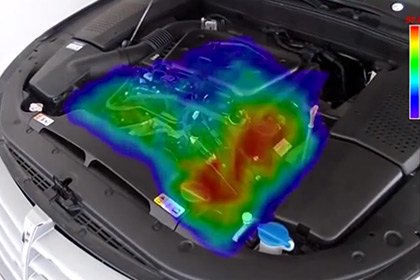
\includegraphics[scale=1]{AcWorkExample.jpg}  
	\caption{Пример работы коммерческого образца акустической камеры}
	\label{fig:AcWorkExample}
\end{figure}

Результат работы акустической камеры обычно выглядит так, как показано на рисунке~\ref{fig:AcWorkExample}

\subsubsection{Применение. }
Существует множество различных применений для акустической камеры, главным из которых является обнаружение источников шума, для их последующего устранения. Камера помогает улучшать шумовые характеристики различных транспортных средств (автомобили, поезда, самолёты) и сооружений (например, турбин). 

С помощью данного устройства, можно не только оценивать характеристики шума излучаемого объектами во внешнюю среду, но улучшать акустический комфорт помещений и кабин транспортных средств.

Поиск причин выхода из строя различных механизмов также можно производить с использованием акустической камеры. Для этого необходимо проанализировать звуковые картины исправного и неисправного механизмов.

Не исключено и военное применение данного устройства. Например, наблюдая за звуковой картиной местности, возможно обнаружить направление, с которого противник ведёт огонь.

В случае разработки дешёвой и компактной акустической камеры не исключено её использование в качестве необычного гаджета.

\subsubsection{Структура и принцип работы. }
Для того, чтобы понять, как работает акустическая камера, взглянем на её функциональную схему, изображённую на рисунке~\ref{fig:AcousticCameraDiagram}. Из данной схемы видно, что вся система состоит из 4 функциональных блоков:
\begin{itemize}
	\item Микрофонная решётка. Данное устройство играет роль датчика, благодаря которому можно определять положение источников звука в пространстве. Более подробная информация о микрофонных решётках приведена в разделе~\ref{section:MicrophoneArrays};
	\item Видеокамера. Это устройство производит съёмку анализируемого объекта и некоторого пространства вокруг него, чтобы построить более понятное человеку изображение. Чаще всего видеокамеру располагают в центре микрофонной решётки, для облегчения задачи совмещения видеоизображения и данных полученных с микрофонной решётки;
	\item Вычислительный модуль служит для анализа данных приходящих с микрофонной решётки и совмещения результатов этого анализа с видеоизображением. Такой анализ можно произвести при помощи пространственной фильтрации, подробнее о которой рассказано в разделе~\ref{section:SpatialFiltering}. Также данный модуль может использоваться для расчётов звукового давления и перевода его в необходимые единицы измерения, если это необходимо;
	\item Устройство вывода необходимо для отображения полученных вычислительным модулем данных. В его качестве можно использовать обычный жидкокристаллический монитор.
\end{itemize}

\begin{figure}[ht]
	\centering
	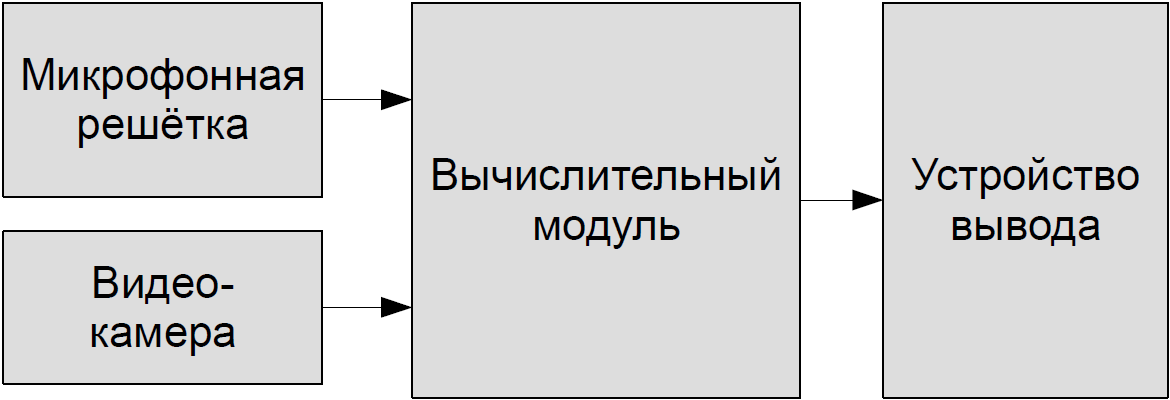
\includegraphics[scale=0.5]{AcousticCameraDiagram.png}  
	\caption{Функциональная схема акустической камеры}
	\label{fig:AcousticCameraDiagram}
\end{figure}

% **************************************************
\subsection{Микрофонные решётки}
\label{section:MicrophoneArrays}
Микрофонная решётка (массив микрофонов)~--- система микрофонов, расположенных определённым образом друг относительно друга. Чаще всего используемые в этой системе микрофоны являются всенаправленными. При дальнейшей обработке данных с такой решётки возможно сформировать заданную диаграмму направленности всей системы без изменения её физических параметров.

\subsubsection{Одномерные решётки. }
Самым простым типом микрофонных решёток является линейная решётка, расположение микрофонов в которой показано на рисунке~\ref{fig:LinearMicArray}. Как видно из рисунка эта решётка является одномерной, следовательно по данным полученным с такой решётки возможно построить лишь одномерную звуковую картину. Однако, несмотря на невозможность построения полноценной двумерной картины, простота конструкции и обработки получаемых с решётки данных, делают такую конфигурацию микрофонов весьма привлекательной для использования в прототипе.

\begin{figure}[ht]
	\centering
	
\includegraphics[scale=1]{MicArrayConfigLinear.png}  
	\caption{Линейная микрофонная решётка}
	\label{fig:LinearMicArray}
\end{figure}

\subsubsection{Двумерные решётки. }
Для того, чтобы построить двумерную карту источников звука, необходимо использовать двуменрные микрофонные решётки.

Двумерные решётки, данные с которых обрабатываются с помощью так называемого бимформинга (см. раздел ~\ref{section:Beamforming}), чаще всего имеют круглую форму. Конфигурации, согласно которым располагают элементы таких решёток обычно бывают следующих типов~\cite[с.~5]{NI_AcousticBeamforming}:
\begin{itemize}
	\item Круговая;
	\item Спиральная;
	\item Случайная.
\end{itemize}

Круговая конфигурация подходит для систем, в которых не известно точное расстояние до источника звука, но при этом ей присущ узкий динамический диапазон. Спиральная конфигурация, даёт лучшие результаты, однако, наилучшие параметры микрофонная решётка имеет при случайном расположении сенсоров. Такое расположение микрофонов позволяет достичь наилучшего динамического диапазона~\cite[с.~5]{NI_AcousticBeamforming}. Примеры описанных конфигураций приведены на рисунке~\ref{fig:MicArrayConfigs}

\begin{figure}[ht]
\centering
  \begin{subfigure}[b]{0.45\textwidth} 
    \centering
    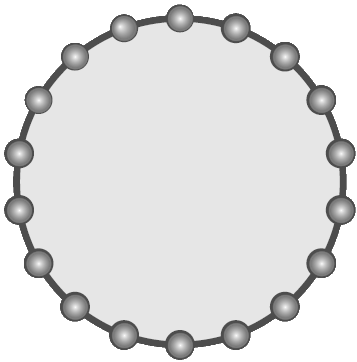
\includegraphics[scale=0.6]{MicArrayConfigRing.png}  
    \caption{}
  \end{subfigure}
  \begin{subfigure}[b]{0.45\textwidth} 
    \centering
    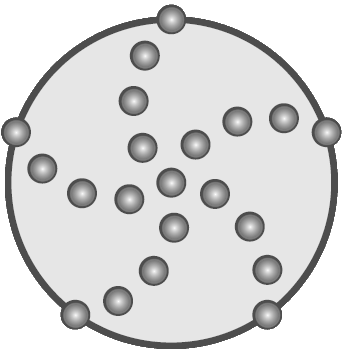
\includegraphics[scale=0.6]{MicArrayConfigSpiral.png}  
    \caption{}
  \end{subfigure}
  \begin{subfigure}[b]{0.45\textwidth} 
    \centering
    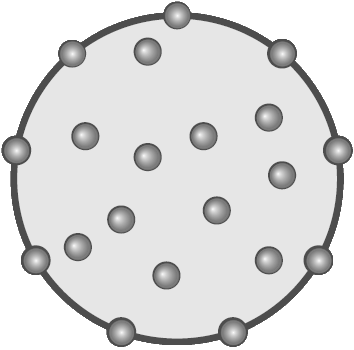
\includegraphics[scale=0.6]{MicArrayConfigRandom.png}  
    \caption{}
  \end{subfigure}
  \caption{ Конфигурации микрофонных решёток:
			а "--- круговая;
            б "--- спиральная;
			в "--- случайная.}
  \label{fig:MicArrayConfigs}
\end{figure}

% **************************************************
\subsection{Пространственная фильтрация}
\label{section:SpatialFiltering}
Пространственная фильтрация~--- процесс выделения сигналов приходящих с желательных направлений и подавления сигналов приходящих с нежелательных направлений из всех сигналов регистрируемых датчиком. 

\begin{figure}[ht]
	\centering
	\includegraphics[scale=0.5]{Screening.png}  
	\caption{Экранирование датчика. Чёрной сплошной стрелкой показан желательный сигнал, а серыми пунктирными нежелательные сигналы.}
	\label{fig:Screening}
\end{figure}

Самым простым способом реализации пространственной фильтрации является экранирование (см. рисунок~\ref{fig:Screening}), при котором сигналы с нежелательных направлений механически изолируются от датчика. Но к сожалению, такой подход имеет существенный недостаток, а именно невозможность изменять диаграмму направленности датчика без изменения физических параметров экрана.

Однако, в последнее время появились и более совершенные подходы к пространственной фильтрации.

\subsection{Бимформинг}
\label{section:Beamforming}
В связи с бурным развитием вычислительной техники и совершенствованием алгоритмов цифровой обработки сигналов, появился новый более гибкий метод пространственной фильтрации, с помощью устройства, которое называется <<бимформер>>. Данный термин является калькой с английского \foreignlanguage{english}{beamformer}, что при дословном переводе означает лучеформирователь.

Бимформер~--- это вычислительное устройство, используемое совместно с массивом датчиков, для выполнения пространственной фильтрации сигналов. Массив датчиков собирает пространственные выборки амплитуды распространяющейся волны, которые обрабатываются бимформером. Главной задачей является оценка направления с которого пришёл желаемый сигнал в присутствии шумов и прочих сигналов интерферирующих с желаемым. Бимформер выполняет пространственную фильтрацию, чтобы разделить сигналы имеющие одинаковые спектральные составляющие, но приходящие с разных направлений~\cite{IEEE_Beamforming}.

Процесс фильтрации с использованием бимформера называют бимформингом.

Выделяют три основных типа бимформинга~\cite{Wiki_SensorArray}:
\begin{itemize}
	\item \dands{} бимформинг
	\item Спектральный бимформинг
	\item Параметрический бимформинг
\end{itemize}
Наиболее простым в реализации, но имеющий худшие характеристики по сравнению с остальными типами является \dands{} бимформинг.

\subsubsection{\dands{} бимформинг. }
\label{section:DelayAndSumBeamforming}
Термин \dands{} при дословном переводе означает задержи и сложи. Принцип работы бимформера, построенного по такой схеме, продемонстрирован на рисунке~\ref{fig:DelayAndSumDiagram}

\begin{figure}[ht]
	\centering
	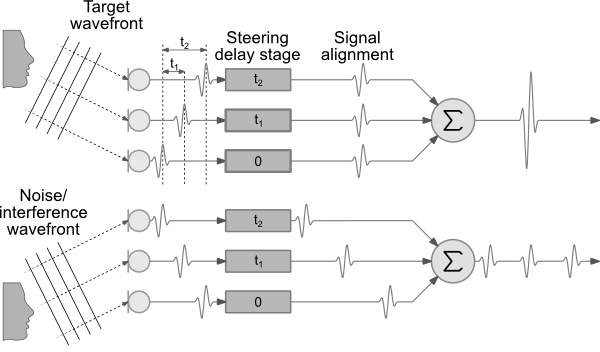
\includegraphics[scale=0.7]{DelayAndSumDiagram.png}  
	\caption{Схема работы \dands{} бимформера}
	\label{fig:DelayAndSumDiagram}
\end{figure}

Данная система состоит из трёх микрофонов, трёх элементов задержки с задержками $0$, $t_1$, $t_2$ и сумматора. Из рисунка можно заметить, что от направления на источник звука зависит разница времени прихода звуковой волны на микрофоны. При фиксированных значениях $t_1$ и $t_2$ звуковой сигнал, приходящий с одного из направлений, будет равен сумме сигналов с трёх микрофонов. Это хорошо видно в верхней части рисунка. В другой части рисунка, сигнал приходит с другого направления, но из-за другой разницы фаз, результирующий сигнал равен сигналу с каждого микрофона в отдельности, а значит, его амплитуда в 3 раза меньше. Таким образом, варьируя значения $t_1$ и $t_2$, можно менять направление, в котором решётка из трёх микрофонов будет наиболее чувствительна.

Применив двумерную решётку и просканировав множество направлений можно построить карту расположения источников звука.

% **************************************************
\subsection{Плотностно-импульсная модуляция}
\label{section:pdm}
Плотностно-импульсная модуляция (\foreignlanguage{english}{pulse-density modulation, PDM}, cигма-дельта модуляция)~--- Способ модуляции используемый для представления аналогового сигнала в цифровой форме. В сигнале закодированном таким образом определённые значения амплитуд не кодируются с помощью слов состоящих из импульсов, имеющих различный вес, как это делается в импульсно-кодовой модуляции. Вместо этого используется относительная плотность импульсов, которая соответствует амплитуде исходного аналогового сигнала~\cite{Wiki_PDM}.

Для того, чтобы понять принцип работы данного вида модуляции, рассмотрим сначала принцип работы дельта-модуляции.

\subsubsection{Дельта-модуляция. }
Рассмотрим блок-схему дельта-модулятора, изображённую на рисунке~\ref{fig:DeltaModulation}.

\begin{figure}[ht]
	\centering
	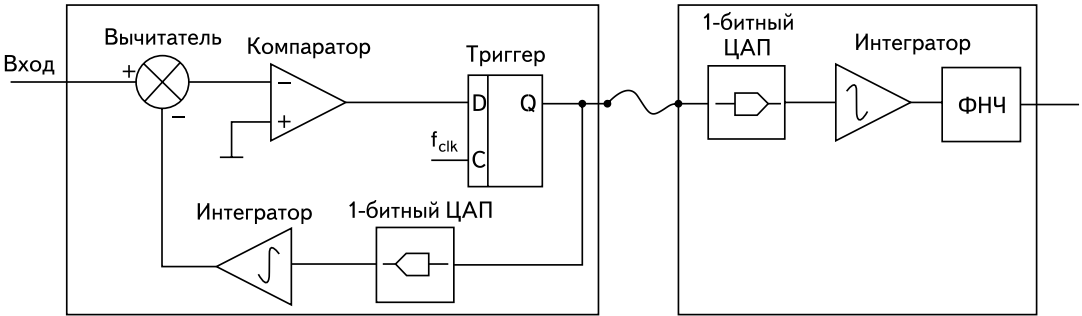
\includegraphics[scale=0.55]{DeltaModulation.png}  
	\caption{Блок-схема дельта-модулятора: ФНЧ~--- фильтр низких частот}
	\label{fig:DeltaModulation}
\end{figure}

Принцип его действия можно описать следующим образом: на основании некоторого набора предыдущих выборок сигнала делается предположение о последующей. Затем предполагаемое значение сравнивается с фактическим и выносится решение о знаке их различия, что и является выходным сигналом~\cite{KitE_DeltaSigma}.

Напряжение входного сигнала подаётся на вычитатель, где из него вычитается аппроксимирующее напряжение, созданное на основании предыдущих значений сигнала. Далее разность поступает на стробируемый компаратор, где сравнивается с нулевым уровнем. Таким образом, логическая единица на выходе компаратора означает, что эта разность положительна или что входной сигнал больше предполагаемого (аппроксимирующего), а логический ноль, соответственно, означает, что входной сигнал меньше аппроксимирующего. Далее последовательность нулей и единиц поступает на однобитный местный ЦАП, который обычно представляет из себя преобразователь уровней одно-полярного напряжения (лог. «0» и лог. «1») в двухполярное ($\pm{}U_{\text{пит}}$). С выхода ЦАП сигнал поступает на вход интегратора, на выходе которого формируется аппроксимирующее напряжение, с заданной точностью повторяющее входное. Точность определяется частотой стробирования компаратора и шагом приращения напряжения в интеграторе. Схема приёмной части состоит из однобитного ЦАП, интегратора и ФНЧ~\cite{KitE_DeltaSigma}.

Эта схема имеет ряд существенных недостатков, которые препятствовали ее применению в аппаратуре аналогово-цифрового преобразования. Попытки её модернизации привели к переходу от дельта-модуляции к дельта-сигма модуляции~\cite{KitE_DeltaSigma}.

\subsubsection{Дельта-сигма модуляция. }
Этот тип модуляции обладает всеми достоинствами дельта-модуляции и в то же время лишён многих её недостатков. Для того чтобы разобраться в его структуре и понять, как был выполнен переход от схемы дельта-модулятора к схеме дельта-сигма модулятора (ДСМ), можно рассуждать следующим образом. Как известно, дельта-модулятор пригоден для работы только с хорошо коррелированными сигналами, поэтому для повышения коррелированности входного сигнала его можно пропустить через интегратор, а на приёмной стороне выходной преобразованный сигнал пропустить, соответственно, через дифференциатор~\cite{KitE_DeltaSigma} (см. рисунок~\ref{fig:DeltaToDeltaSigma}).

\begin{figure}[ht]
	\centering
	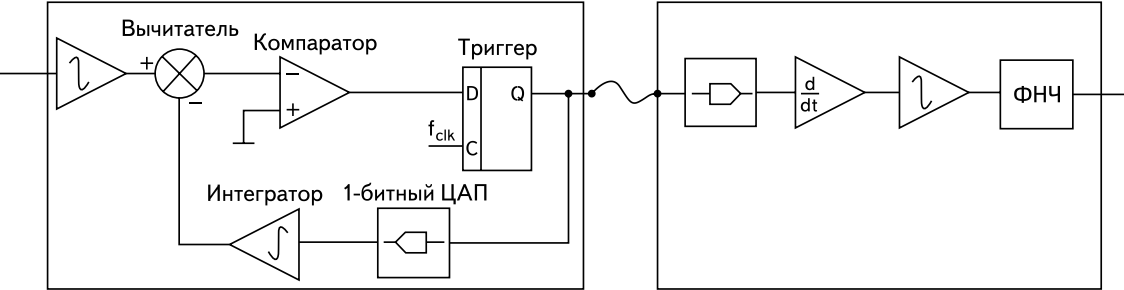
\includegraphics[scale=0.55]{DeltaToDeltaSigma.png}  
	\caption{Переход от дельта-модулятора к дельта-сигма модулятору}
	\label{fig:DeltaToDeltaSigma}
\end{figure}

Поскольку разность интегралов равна интегралу разности, то два интегратора на входах вычитателя можно заменить одним на его выходе. Что касается дифференциатора на приёмной стороне, то он вместе с приёмным интегратором может быть исключён. Таким образом, схема ДСМ, изображённая на рисунке~\ref{fig:DeltaSigmaModulation}, отличается от дельта-модулятора положением интегратора на передающей стороне и его отсутствием на приёмной. Такое незначительное изменение в схеме значительно улучшило её характеристики и, в частности, позволило достичь отношения сигнал/шум -120 дБ~\cite{KitE_DeltaSigma}.

\begin{figure}[ht]
	\centering
	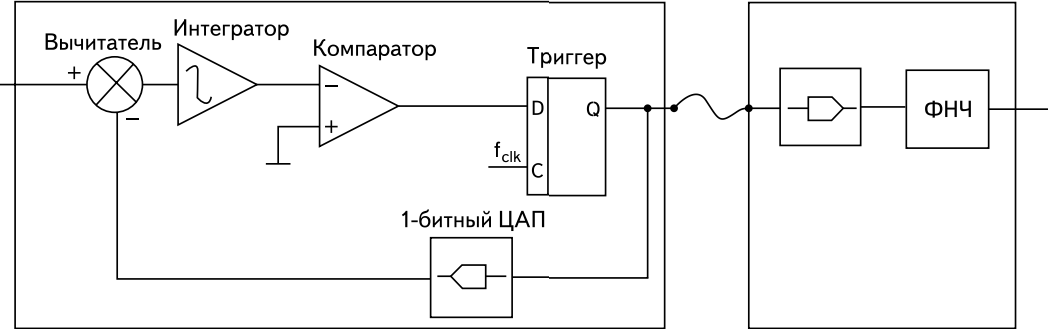
\includegraphics[scale=0.55]{DeltaSigmaModulation.png}  
	\caption{Схема дельта-сигма модулятора}
	\label{fig:DeltaSigmaModulation}
\end{figure}

Рассмотрим работу схемы ДСМ. Когда образуется высококоррелированный сигнал, то коррелированными оказываются не только его отсчёты, но и ошибки при каждом квантовании. Следовательно, их легко предсказать и вычесть из сигнала, отправляемого на устройство квантования, прежде чем произойдёт квантование. Хорошей оценкой текущей ошибки в таком случае выступает предшествующая ошибка. Предшествующая ошибка, образованная как разность между входом и выходом устройства квантования, помещается в схему задержки (триггер). Таким образом, в контуре обратной связи циркулирует сигнал ошибки~\cite{KitE_DeltaSigma}.

Выходной сигнал ДСМ представляет собой однобитный поток импульсов. Рассмотрим его в терминах теории вероятности. Так, вероятность появления в потоке логической единицы $P(1)$ и вероятность появления логического нуля $P(0)$ связаны следующим выражением: $P(0)+P(1) = 1$. Более того, если на вход модулятора подаётся некий сигнал (ограниченный в динамическом диапазоне 0~--~1), то вероятность $P(1)=x$, а $P(0)=(1-x)$. Иными словами, чем плотнее представлены импульсы определённой полярности в потоке, тем выше уровень сигнала в этот момент. Нулевой уровень сигнала кодируется одинаковой плотностью положительных и отрицательных импульсов. Импульсные последовательности при кодировании синусоидального напряжения представлены на рисунке~\ref{fig:DeltaSigmaOscillogram}. Видно, что плотность положительных и отрицательных импульсов одинакова в точках, близких к 0, плотность отрицательных импульсов максимальна в точке $-1$, и плотность положительных импульсов максимальна в точке $+1$~\cite{KitE_DeltaSigma}.

\begin{figure}[ht]
	\centering
	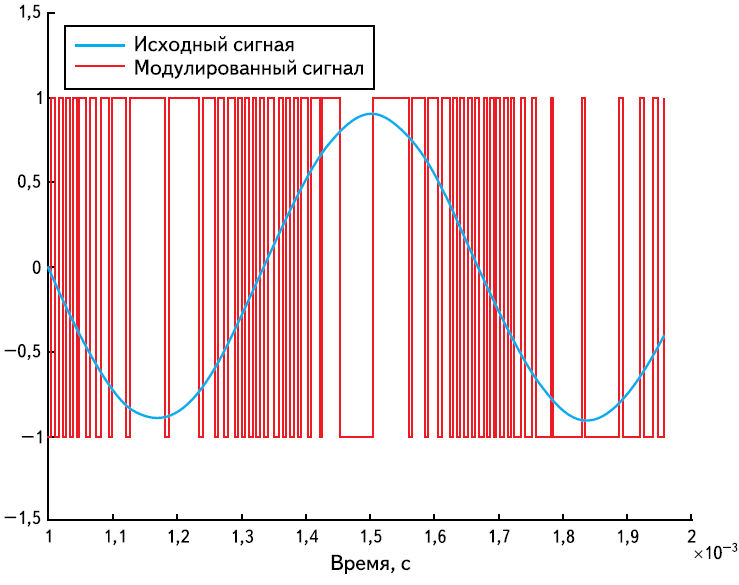
\includegraphics[scale=0.8]{DeltaSigmaOscillogram.png}  
	\caption{Осциллограмма выходного сигнала дельта-сигма модулятора}
	\label{fig:DeltaSigmaOscillogram}
\end{figure}

Такие особенности позволяют кодировать в формате дельта-сигма модуляции сигналы с частотой от 0 до 100 кГц. В частности, прямоугольное аналоговое напряжение и уровни постоянного напряжения, последнее актуально при применении дельта-сигма модуляции в датчиках медленно меняющихся сигналов~\cite{KitE_DeltaSigma}.

\begin{figure}[ht]
\centering
  \begin{subfigure}[b]{0.45\textwidth} 
    \centering
    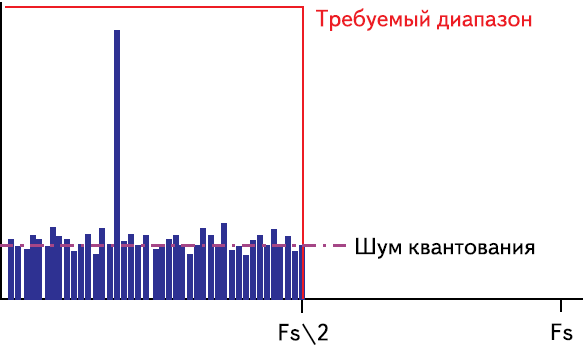
\includegraphics[scale=0.45]{OutputSpectrumA.png}  
    \caption{}
  \end{subfigure}
  \begin{subfigure}[b]{0.45\textwidth} 
    \centering
    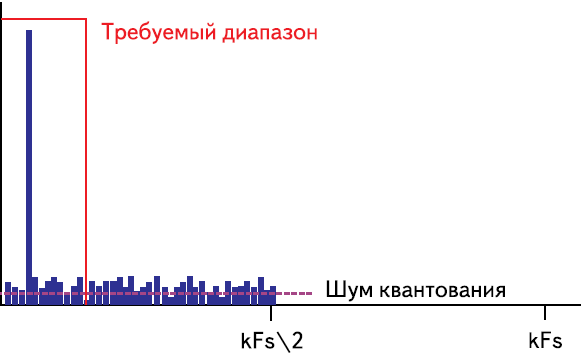
\includegraphics[scale=0.45]{OutputSpectrumB.png}  
    \caption{}
  \end{subfigure}
  \begin{subfigure}[b]{0.45\textwidth} 
    \centering
    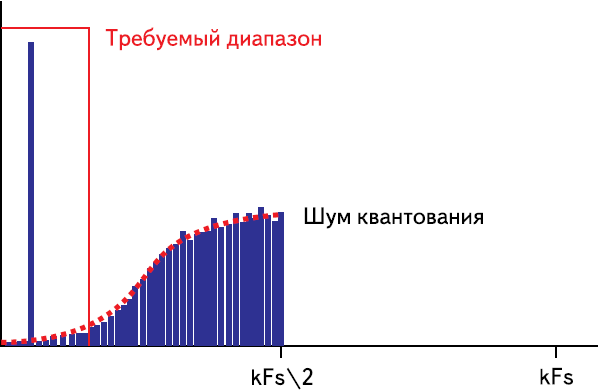
\includegraphics[scale=0.45]{OutputSpectrumC.png}  
    \caption{}
  \end{subfigure}
  \caption{ Спектры выходного сигнала:
			а "--- при обычных условиях;
            б "--- при оверсемплинге;
			в "--- при использовании нойзшейпинга.}
  \label{fig:OutputSpectrum}
\end{figure}

\subsubsection{Шумы. }
Исследование шумов в ДСМ заслуживает отдельного рассмотрения. Ведь методы достижения отношения сигнал/шум -120 дБ при разрядности 1 бит представляют известный интерес. В 1954 году С. Катлер из той же лаборатории Александра Бэлла предложил концепцию передискретизации и формирования спектра шума. Как известно, каждый дополнительный бит при преобразовании аналогового сигнала в цифровой добавляет 6 дБ к отношению сигнал/шум (рисунок~\ref{fig:OutputSpectrum}a). Одним из основополагающих принципов дельта-модуляции является превышение частоты Котельникова в К раз. При такой передискретизации эффективная разрядность, а соответственно, и отношение сигнал/шум, увеличивается согласно формуле $K=2^N$, где $K$~--- коэффициент передискретизации, а $N$~--- количество дополнительных битов. Обычно применяется $K=64$, и в этом случае эффективная разрядность будет 7 бит, а отношение сигнал/шум будет равно 42 дБ (рисунок~\ref{fig:OutputSpectrum}б). Однако передискретизация сама по себе не является эффективным средством. Дальнейшее подавление шума производится благодаря самой структуре дельта-сигма модулятора. В иностранной литературе часто применяется термин <<нойзшейпинг>> (англ. \foreignlanguage{english}{noise shaping}), что означает формирование спектра шума. Чтобы понять, как именно происходит формирование, используем линеаризованную дискретную модель системы, в которой входной сигнал представлен последовательностью $x(n)$, выходной сигнал $y(x)$ и шум квантования, вносимый компаратором и триггером,~--- $e(n)$, что изображено на рисунке~\ref{fig:DeltaSigmaLinearModel}~\cite{KitE_DeltaSigma}.

\begin{figure}[ht]
	\centering
	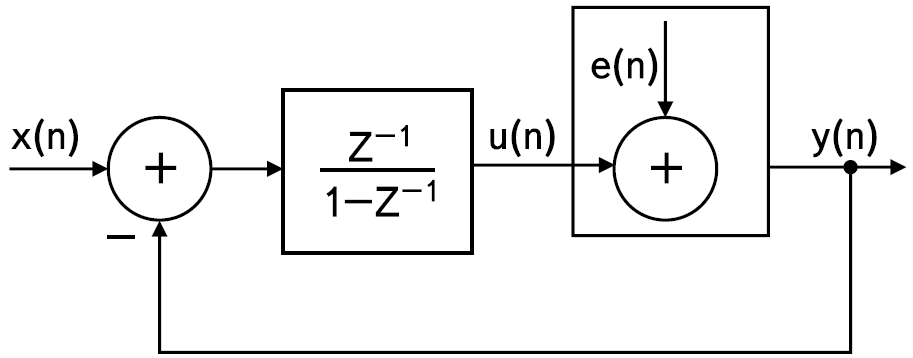
\includegraphics[scale=0.6]{DeltaSigmaLinearModel.png}  
	\caption{Осциллограмма выходного сигнала дельта-сигма модулятора}
	\label{fig:DeltaSigmaLinearModel}
\end{figure}

Рассмотрим Z-преобразование этой системы дельта-сигма модулятора:

\begin{gather}
	Y(z)=\frac{X(z)-Y(z)}{z\left(1-\frac{1}{z}\right)}+E(z), \\
	Y(z)=\frac{X(z)}{z}+\left(1-\frac{1}{z}\right)E(z).
\end{gather}

Видно, что полезный сигнал $X(z)$ проходит эту цепь без изменений, с задержкой на 1 такт, в то время как для шума возникает препятствие в виде ФНЧ. Таким образом, осуществляется формирование спектра шума в дельта-сигма модуляторе. Интегратор в данном случае выступает в качестве ФНЧ для шумовой составляющей сигнала. Энергия шума сосредотачивается в области верхних частот, и большая ее часть может быть отфильтрована выходным ФНЧ (рисунок~\ref{fig:OutputSpectrum}в). Таким образом, в выходном сигнале после демодулирования дельта-сигма последовательности наблюдается намного более низкий уровень шума, чем можно было бы предполагать. Следующим шагом по улучшению параметров по шумам является повышение порядка модулятора. Следует особо отметить, что дельта-сигма АЦП с высочайшей (24 бита) эффективной разрядностью можно построить, всего лишь используя интегратор и стробируемый компаратор~\cite{KitE_DeltaSigma}.

\subsubsection{Информационные параметры. }
Еще одним важным на сегодня параметром сигнала является его информационная ёмкость. Здесь следует отметить, что сигнал в формате дельта-сигма модуляции не требует кадровой синхронизации, а значит, считывать его можно в любой момент времени в записи или в канале передачи. В этом его сходство с аналоговым сигналом. Ещё одно важное его отличие~--- это факт одинаковой информационной ёмкости каждого бита в потоке, что повышает помехоустойчивость сигнала в формате дельта-сигма модуляции~\cite{KitE_DeltaSigma}.

Оценим теперь информационные параметры сигнала. В качестве требуемого диапазона возьмем порог слышимости, принятый в различных стандартах звукозаписи,~--- 22 кГц. Частота Котельникова в ИКМ для такого диапазона, следовательно, будет равняться 44 кГц. Оверсэмплинг в формате дельта-сигма модуляции (например, SACD фирмы Sony) предполагает 64-кратное увеличение частоты Котельникова. Таким образом, получается, что частота дискретизации в формате дельта-сигма модуляции с овер-сэмплингом будет равна 2,82 МГц для передачи диапазона от 0 до 22 кГц. Учитывая, что передача цифровых сигналов в обоих форматах ведётся в последовательном режиме, оценим количество бит в секунду. При последовательной передаче в формате ИКМ 44 кГц/16 бит поток равен 705 кБод, в формате дельта-модуляции~--- 2,8 мБод. Однако качество сигнала в формате дельта-модуляции 2,8 МГц приближается к качеству сигнала в формате ИКМ~--- 192 кГц/24 бита, поток которого составляет уже 4,8 мБод. Также следует учесть, что, в отличие от дельта-сигма модуляции, при передаче ИКМ-сигналов требуется жёсткая кадровая синхронизация~\cite{KitE_DeltaSigma}.

% **************************************************
\subsection{Общие сведения о цифровых фильтрах}
\label{section:DigitalFilters}
Цифровой фильтр~--- в электронике любой фильтр, обрабатывающий цифровой сигнал с целью выделения и/или подавления определённых частот этого сигнала. В отличие от цифрового, аналоговый фильтр имеет дело с аналоговым сигналом, его свойства недискретны, соответственно передаточная функция зависит от внутренних свойств составляющих его элементов~\cite{Wiki_DigitalFilter}.

\subsubsection{Применение. }
Цифровые фильтры на сегодняшний день применяются практически везде, где требуется обработка сигналов, в частности в спектральном анализе, обработке изображений, обработке видео, обработке речи и звука и многих других приложениях~\cite{Wiki_DigitalFilter}.

\subsubsection{Характеристика цифровых фильтров. }
Линейный стационарный цифровой фильтр характеризуется передаточной функцией. Передаточная функция может описать, как фильтр будет реагировать на входной сигнал. Таким образом, проектирование фильтра состоит из постановки задачи (например, фильтр восьмого порядка, фильтр нижних частот с конкретной частотой среза), а затем производится расчёт передаточной функции, которая определяет характеристики фильтра~\cite{Wiki_DigitalFilter}.

Передаточная функция фильтра имеет вид:
\begin{equation}
	H(z)=\frac{B(z)}{A(z)}=\frac{b_0+b_1z^{-1}+b_2z^{-2}+...+b_Nz^{-N}}{1+a_1z^{-1}+a_2z^{-2}+...+a_Mz^{-M}},
\end{equation}
\begin{explanation}
	где & порядок фильтра & большее $N$ или $M$.
\end{explanation}
В данном случае это формула БИХ-фильтра. Если знаменатель равен единице, то получаем формулу КИХ-фильтра (без обратной связи)~\cite{Wiki_DigitalFilter}.

\subsubsection{Преимущества. }
Преимуществами цифровых фильтров перед аналоговыми являются~\cite{Wiki_DigitalFilter}:
\begin{itemize}
	\item Высокая точность (точность аналоговых фильтров ограничена допусками на элементы);
	\item Стабильность (в отличие от аналогового фильтра передаточная функция не зависит от дрейфа характеристик элементов);
	\item Гибкость настройки, лёгкость изменения;
	\item Компактность~--- аналоговый фильтр на очень низкую частоту (доли герца, например) потребовал бы чрезвычайно громоздких конденсаторов или индуктивностей.
\end{itemize}

\subsubsection{Недостатки. }
Недостатками цифровых фильтров по сравнению с аналоговыми являются~\cite{Wiki_DigitalFilter}:
\begin{itemize}
	\item Трудность работы с высокочастотными сигналами. Полоса частот ограничена частотой Найквиста, равной половине частоты дискретизации сигнала. Поэтому для высокочастотных сигналов применяют аналоговые фильтры, либо, если на высоких частотах нет полезного сигнала, сначала подавляют высокочастотные составляющие с помощью аналогового фильтра, затем обрабатывают сигнал цифровым фильтром;
	\item Трудность работы в реальном времени — вычисления должны быть завершены в течение периода дискретизации;
	\item Для большой точности и высокой скорости обработки сигналов требуется не только мощный процессор, но и дополнительное, возможно дорогостоящее, аппаратное обеспечение в виде высокоточных и быстрых ЦАП и АЦП.
\end{itemize}

\subsubsection{Виды. }
Цифровые фильтры подразделяют на два основных класса:
\begin{itemize}
	\item КИХ-фильтры
	\item БИХ-фильтры
\end{itemize}

% **************************************************
\subsection{Фильтр с бесконечной импульсной характеристикой}
\label{section:IIR}
Фильтр с бесконечной импульсной характеристикой (рекурсивный фильтр, БИХ-фильтр) или IIR-фильтр (IIR сокр. от англ. \foreignlanguage{english}{infinite impulse response}~--- бесконечная импульсная характеристика)~--- линейный электронный фильтр, использующий один или более своих выходов в качестве входа, то есть образует обратную связь. Основным свойством таких фильтров является то, что их импульсная переходная характеристика имеет бесконечную длину во временной области, а передаточная функция имеет дробно-рациональный вид. Такие фильтры могут быть как аналоговыми, так и цифровыми~\cite{Wiki_IIR}.

Примерами БИХ-фильтров являются~\cite{Wiki_IIR}:
\begin{itemize}
	\item Фильтр Чебышёва;
	\item Фильтр Баттерворта;
	\item Фильтр Калмана;
	\item Фильтр Бесселя.
\end{itemize}

\subsubsection{Динамические характеристики. }
Разностное уравнение, описывающее дискретный БИХ-фильтр, устанавливает связь между входным и выходным сигналами во временной области:
\begin{eqnarray}
	y(n) = b_{0} x(n) + b_{1} x(n-1) + \cdots + b_{P} x(n-P) - \nonumber \\
	- a_{1} y(n-1) - a_{2} y(n-2) - \cdots - a_{Q} y(n-Q),
\end{eqnarray}
\begin{explanation}
	где &$P$& порядок входного сигнала; \\
	&$b_{i}$& коэффициенты входного сигнала; \\
	&$Q$& порядок обратной связи; \\
	&$a_{i}$& коэффициенты обратной связи; \\
	&$x(n)$& входной сигнал; \\
	&$y(n)$& выходной сигнал; \\
\end{explanation}
Более компактная запись разностного уравнения:
\begin{equation}
	y(n) = \sum_{i=0}^P b_{i}x(n-i) - \sum_{k=1}^Q a_{k} y(n-k).
\end{equation}
Для того, чтобы найти ядро фильтра, положим:
\begin{equation}
	x(n) = \delta(n),
\end{equation}
\begin{explanation}
	где &$\delta(n)$& дельта-функция.
\end{explanation}
Тогда импульсная переходная функция (ядро фильтра) записывается как:
\begin{equation}
	h(n)=\sum_{i=0}^P b_{i}\delta(n-i) - \sum_{k=1}^Q a_{k} h(n-k).
\end{equation}
Z-преобразование импульсной переходной функции даёт передаточную функцию БИХ-фильтра~\cite{Wiki_IIR}:
\begin{equation}
	H(z)= \frac{\sum_{i=0}^P b_{i} z^{-i}}{1+\sum_{k=1}^Q a_{k} z^{-k}}.
\end{equation}

\subsubsection{Устойчивость. }
Об устойчивости фильтра с бесконечной импульсной характеристикой судят по его передаточной функции. Для дискретного фильтра необходимо и достаточно, чтобы все полюса его передаточной функции по модулю были меньше единицы (т. е. лежали внутри единичного круга на z-плоскости). Все критерии устойчивости, применимые в теории линейных стационарных систем, например критерий устойчивости Найквиста или критерий устойчивости Рауса применимы и в случае БИХ-фильтров~\cite{Wiki_IIR}.

В отличие от КИХ-фильтров, БИХ-фильтры не всегда являются устойчивыми~\cite{Wiki_IIR}.

\subsubsection{Реализация БИХ фильтра. }
Если рассматривается передаточная функция вида:
\begin{equation}
	H(z) = \frac{Y(z)}{X(z)} = \frac{\sum_ {k=0}^{M} b_{k} z ^{-k} } { 1 + \sum_ {k=1}^{N} a_{k} z ^{-k}} = \frac{B(z)}{A(z)}, 
\end{equation}
то соотношение между входом и выходом такой системы должно удовлетворять разностному уравнению:
\begin{equation}
	y(n) = -\sum_ {k=1}^N a(k)y(n - k) + \sum_ {k=0}^M b(k)x(n - k).
\end{equation}
Это уравнение может быть записано непосредственно из выражения для передаточной функции, таким образом форму построения цепи, соответствующей этому уравнению, называют прямой формой I~\cite{Wiki_IIR}.

При построении БИХ фильтра для простоты можно принять, что $M=N$. БИХ фильтры могут быть реализованы с использованием трёх элементов или основных операций: умножитель, сумматор и блок задержки. Этих элементов достаточно для всех возможных цифровых фильтров. вариант, показанный на рисунке~\ref{fig:IirDirectFormI} есть прямая реализация БИХ-фильтров типа I. Поскольку совокупности коэффициентов $b(k)$ и $a(k)$ соответствуют полиномам числителя $B(z)$ и знаменателя $A(z)$ передаточной функции $H(z)$, то прямую форму БИХ-фильтра, показанную на рисунке~\ref{fig:IirDirectFormI}, можно трактовать как каскадное соединение двух цепей. Первая из них реализует нули и имеет передаточную функцию $B(z)$, а вторая~--- полюсы, и имеет передаточную функцию $\frac{1}{A(z)}$. Обозначив выходной сигнал первой системы $w(n)$, разностное уравнение можно заменить системой уравнений~\cite{Wiki_IIR}:
\begin{gather}
	y(n) = - \sum_ {k=1}^{N} a(k)y(n - k) + w(n), \\
	w(n) = \sum_ {k=0}^{M} b(k)x(n - k).
\end{gather}
которая и реализована структурой, показанной на рисунке~\ref{fig:IirDirectFormIINonCanonical}.

\begin{figure}[ht]
	\centering
	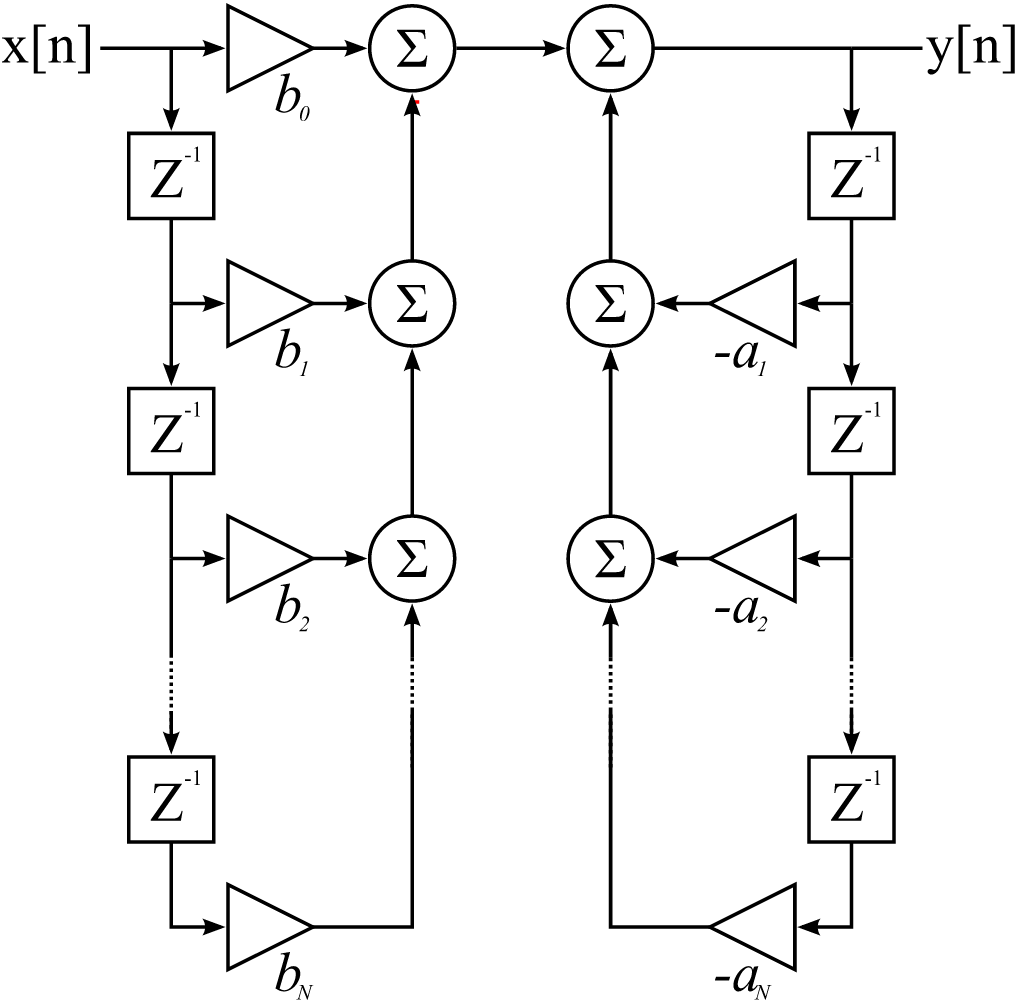
\includegraphics[scale=0.6]{IirDirectFormI.png}  
	\caption{Прямая реализация типа I БИХ фильтра}
	\label{fig:IirDirectFormI}
\end{figure}

\begin{figure}[ht]
	\centering
	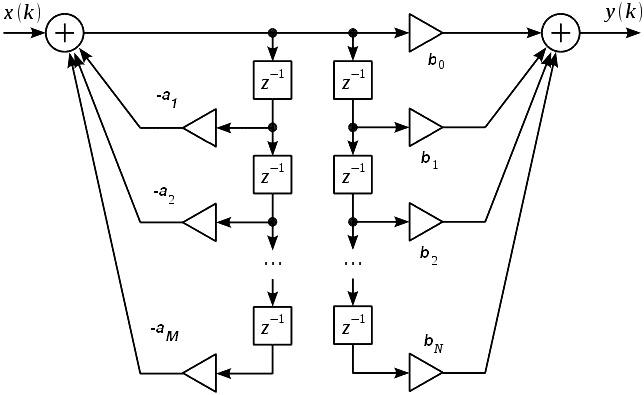
\includegraphics[scale=0.95]{IirDirectFormIINonCanonical.png}  
	\caption{Прямая реализация типа II БИХ фильтра (неканоническая)}
	\label{fig:IirDirectFormIINonCanonical}
\end{figure}

\begin{figure}[ht]
	\centering
	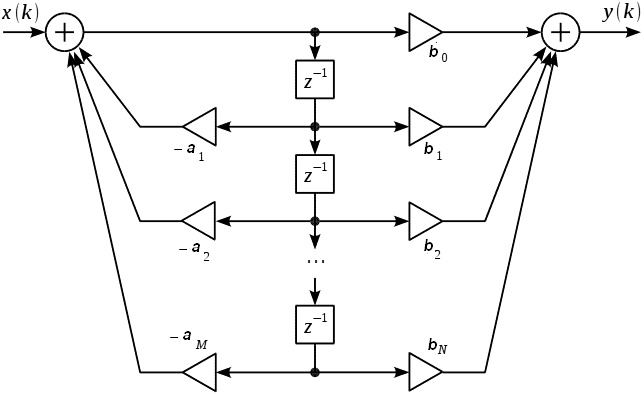
\includegraphics[scale=0.95]{IirDirectFormIICanonical.png}  
	\caption{Прямая реализация типа II БИХ фильтра (каноническая)}
	\label{fig:IirDirectFormIICanonical}
\end{figure}

В дискретных системах с постоянными параметрами соотношение между входом и выходом не зависит от порядка каскадного соединения блоков. Из этого свойства вытекает вторая прямая форма построения БИХ-фильтра. Если сначала реализовать полюсы $H(z)$ соответствующие правой части структурной схемы рисунка~\ref{fig:IirDirectFormI}, которая имеет передаточную функцию $\frac{1}{A(z)}$, а после~--- нули передаточной функцией $B(z)$, то получим структуру, показанную на рисунке~\ref{fig:IirDirectFormIINonCanonical}, которая соответствует системе уравнений~\cite{Wiki_IIR}:
\begin{gather}
	w(n) = -\sum_ {k=1}^{N} a(k)w(n - k) + x(n), \\
	y(n) = \sum_ {k=0}^{M} b(k)w(n - k).
\end{gather}

Объединив линии задержки в структуре, показанной на рисунке~\ref{fig:IirDirectFormIINonCanonical}, получим прямую каноническую форму, показанную на рисунке~\ref{fig:IirDirectFormIICanonical}~\cite{Wiki_IIR}.

В некоторых случаях, с точки зрения шумовых характеристик, фильтр, реализованный в первой прямой форме, лучше, чем в канонической~\cite{Wiki_IIR}.

% **************************************************
\subsection{Фильтр с конечной импульсной характеристикой}
\label{section:FIR}
Фильтр с конечной импульсной характеристикой (нерекурсивный фильтр, КИХ-фильтр) или FIR-фильтр (FIR сокр. от англ. \foreignlanguage{english}{finite impulse response}~--- конечная импульсная характеристика)~--- один из видов линейных цифровых фильтров, характерной особенностью которого является ограниченность по времени его импульсной характеристики (с какого-то момента времени она становится точно равной нулю). Такой фильтр называют ещё нерекурсивным из-за отсутствия обратной связи. Знаменатель передаточной функции такого фильтра~--- некая константа~\cite{Wiki_FIR}.

\subsubsection{Динамические характеристики. }
Разностное уравнение, описывающее связь между входным и выходным сигналами фильтра~\cite{Wiki_FIR}:
\begin{equation}
	y(n) = b_0 x(n) + b_1 x(n-1) +...+ b_P x(n-P),
\end{equation}
где $P$ — порядок фильтра, $x(n)$ — входной сигнал, $y(n)$ — выходной сигнал, а $b_{i}$ — коэффициенты фильтра. Иными словами, значение любого отсчёта выходного сигнала определяется суммой масштабированных значений $P$ предыдущих отсчётов. Можно сказать иначе: значение выхода фильтра в любой момент времени есть значение отклика на мгновенное значение входа и сумма всех постепенно затухающих откликов $P$ предыдущих отсчётов сигнала, которые всё ещё оказывают влияние на выход (после $P$-отсчётов импульсная переходная функция становится равной нулю, как уже было сказано, поэтому все члены после $P$-го тоже станут равными нулю). Запишем предыдущее уравнение в более ёмком виде:
\begin{equation}
	y(n) = \sum_{i=0}^{P} b_i x(n-i).
\end{equation}
Для того, чтобы найти ядро фильтра, положим:
\begin{equation}
	x(n) = \delta(n),
\end{equation}
\begin{explanation}
	где &$\delta(n)$& дельта-функция.
\end{explanation}
Тогда импульсная характеристика КИХ-фильтра может быть записана как:
\begin{equation}
	h(n) = \sum_{i=0}^{P}b_i \delta(n-i).
\end{equation}
Z-преобразование импульсной характеристики даёт нам передаточную функцию КИХ-фильтра~\cite{Wiki_FIR}:
\begin{equation}
	H(z) = \sum_{i=0}^{P}b_i z^{-i}.
\end{equation}

\subsubsection{Свойства. }
КИХ-фильтр обладает рядом полезных свойств, из-за которых он иногда более предпочтителен в использовании, чем БИХ-фильтр. Вот некоторые из них~\cite{Wiki_FIR}:
\begin{itemize}
	\item КИХ-фильтры устойчивы;
	\item КИХ-фильтры при реализации не требуют наличия обратной связи;
	\item Фаза КИХ-фильтров может быть сделана линейной.
\end{itemize}

\subsubsection{Прямая форма КИХ-фильтра. }
КИХ-фильтры могут быть реализованы с использованием трёх элементов: умножитель, сумматор и блок задержки. Вариант, показанный на рисунке~\ref{fig:FirStructure}, есть прямая реализация КИХ-фильтров типа I~\cite{Wiki_FIR}.

\begin{figure}[ht]
	\centering
	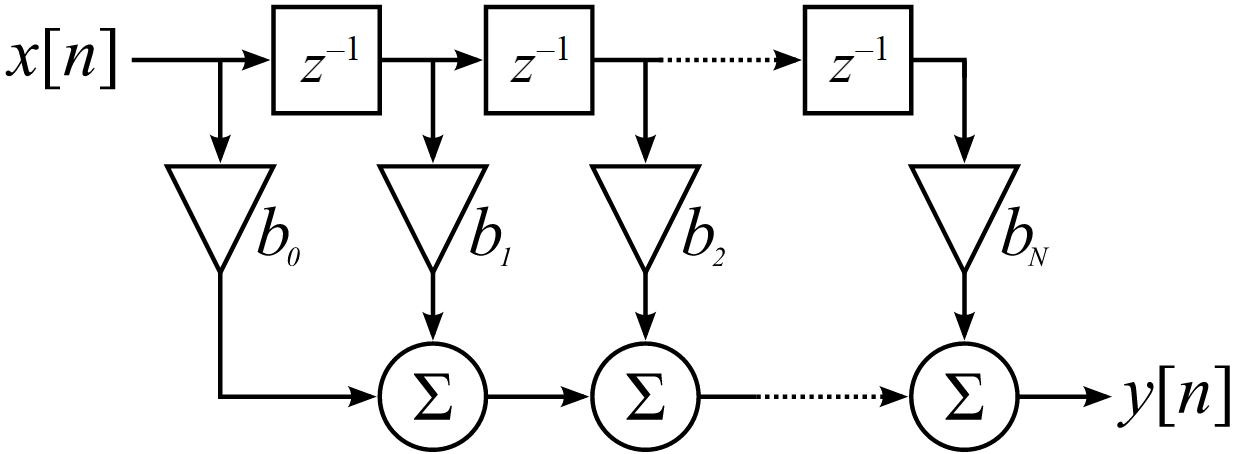
\includegraphics[scale=0.45]{FirStructure.png}  
	\caption{Реализация прямой формы КИХ-фильтра}
	\label{fig:FirStructure}
\end{figure}
\section{Используемые компоненты и технологии}
\label{section:Technologies}

% **************************************************
\subsection{PDM микрофон \micname{}}
На данный момент существует огромное число различных видов микрофонов с широким спектром характеристик. Но большинство из них мало подходят для применения в микрофонных решётках. Дело в том, что обычные микрофоны выдают на выходе аналоговый сигнал и для его последующей цифровой обработки потребуется АЦП. С ростом числа микрофонов в решётке возрастёт и число микросхем АЦП, что приведёт к удорожанию и усложнению конечного устройства.

Однако, в последнее время, на рынке появились, так называемые, цифровые микрофоны. Они имеют интегрированный АЦП и выдают на выходе сигнал в PDM формате. Примером такого устройства является микрофон \micname{} от фирмы ST. Его внешний вид представлен на рисунке~\ref{fig:PdmMicPhoto}

\begin{figure}[ht]
	\centering
	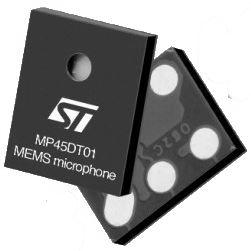
\includegraphics[scale=1.2]{PdmMicPhoto.jpg}  
	\caption{Микрофон \micname{}}
	\label{fig:PdmMicPhoto}
\end{figure}

\subsubsection{Возможности. }
Фирма ST заявляет следующие возможности микрофона \micname~\cite{ST_MP45DT02}:
\begin{itemize}
	\item Для работы необходимо только одно напряжения питания;
	\item Низкая потребляемая мощность при работе;
	\item Всенаправленная чувствительность;
	\item Однобитный выход с возможностью работы в стерео-режиме;
	\item Металлический или пластиковый HLGA корпус для поверхностного монтажа.
\end{itemize}

\subsubsection{Характеристики. }
Микрофон \micname{} обладает следующими характеристиками~\cite{ST_MP45DT02}:
\begin{itemize}
	\item Напряжение питания 1,64--3,6 В;
	\item Потребляемый ток в рабочем режиме 0,65 мА;
	\item Отношение сигнал-шум 61 дБ;
	\item Чувствительность -26 дБ;
	\item Максимальная тактовая частота 3,25 МГц.
\end{itemize}

Амплитудно-частотная характеристика данного микрофона изображена на рисунке~\ref{fig:PdmMicResponse}

\begin{figure}[ht]
	\centering
	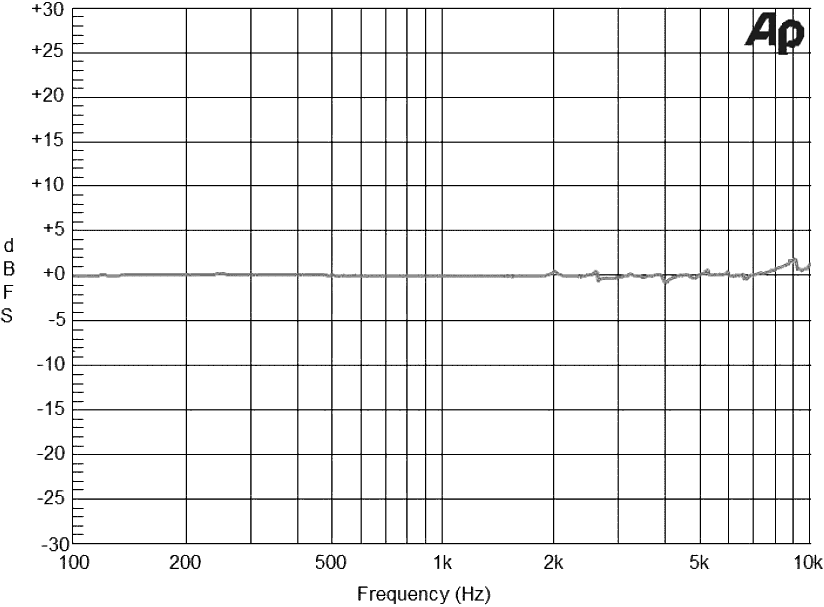
\includegraphics[scale=0.75]{PdmMicResponse.png}  
	\caption{Амплитудно-частотная характеристика микрофона \micname{}}
	\label{fig:PdmMicResponse}
\end{figure}

\subsubsection{Применение. }
Микрофон \micname{} может применяться в таких областях как~\cite{ST_MP45DT02}:
\begin{itemize}
	\item Мобильные терминалы;
	\item Ноутбуки и портативные компьютеры;
	\item IP-телефония;
	\item Распознавание речи;
	\item Игровые устройства и устройства виртуальной реальности;
	\item Цифровые видеокамеры;
	\item Охранные системы.
\end{itemize}

\subsubsection{Краткое описание. }
\micname{}~--- это компактный, потребляющий небольшое количество энергии, всенаправленный микрофон с верхним расположением звукового отверстия. В данный микрофон встроен чувствительный элемент и цифровой интерфейс с возможностью работы в стерео-режиме~\cite{ST_MP45DT02}.

Чувствительный элемент, способный регистрировать акустические волны, произведён с использованием специального процесса микрообработки кремния~\cite{ST_MP45DT02}.

Встроенная интегральная микросхема, произведённая по CMOS технологии, позволяет получать с микрофона сигнал в PDM формате~\cite{ST_MP45DT02}.

\micname{} имеет акустическую точку перегрузки в 120 дБ с лучшим на рынке отношением сигнал/шум 61 дБ и чувствительностью $-20$~дБ
Встроенная интегральная микросхема, произведённая по CMOS технологии, позволяет получать с микрофона сигнал в PDM формате~\cite{ST_MP45DT02}.

\micname{} доступен в SMD-совместимом металлическом либо пластиковом корпусе с гарантией функционирования в расширенном диапазоне температур от $-30\,^{\circ}{\rm C}$ до $85\,^{\circ}{\rm C}$~\cite{ST_MP45DT02}.

Цифровой выход и небольшие размеры корпуса (толщина всего 1,25~мм) делают данный микрофон наилучшим решением для переносных вычислительных устройств~\cite{ST_MP45DT02}.

\subsubsection{Схема подключения. }
Каждый микрофон \micname{} оснащён последовательным интерфейсом для считывания данных в формате PDM.
 
Данный последовательный интерфейс состоит из входа для тактирования цифровой части микрофона и выходом данных. Для возможности подключения двух микрофонов на одну шину данных в микрофоне \micname{} предусмотрен конфигурационный вход, позволяющий задавать момент, когда на выходе данных микрофона появится информация. Согласно документации на микрофон~\cite{ST_MP45DT02}, при подаче на конфигурационный вход логической единицы, данные будут появляться на выходе по переднему фронту тактового сигнала. При подаче на конфигурационный вход логического нуля, данные появятся по заднему фронту тактового сигнала (рисунок~\ref{fig:PdmMicWaveform})
 
\begin{figure}[ht]
	\centering
	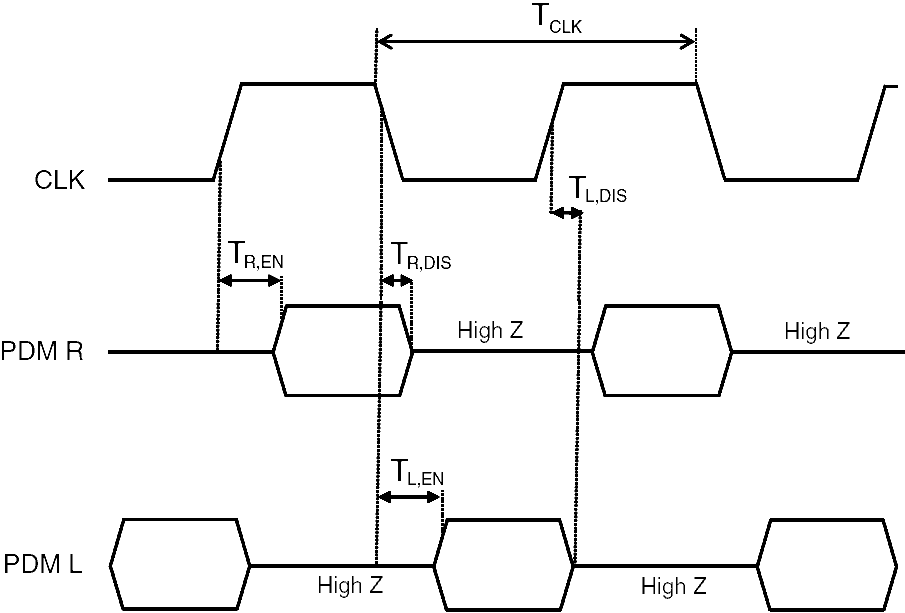
\includegraphics[scale=0.6]{PdmMicWaveform.png}  
	\caption{Форма тактового и выходного сигнала микрофона \micname{}}
	\label{fig:PdmMicWaveform}
\end{figure}
 
Типичная схема подключения двух микрофонов на одну шину данных показана на рисунке~\ref{fig:DoublePdmMic}

\begin{figure}[ht]
	\centering
	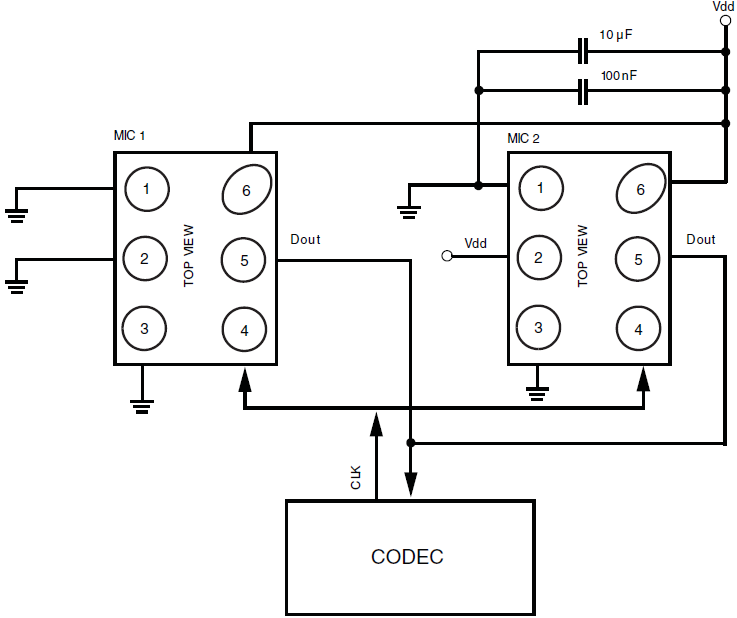
\includegraphics[scale=0.7]{DoublePdmMic.png}  
	\caption{Схема подключения двух микрофонов на одну шину данных}
	\label{fig:DoublePdmMic}
\end{figure}


% **************************************************
\subsection{Программируемые пользователем вентильные матрицы}

Программируемая логическая интегральная схема (ПЛИС, англ. \foreignlanguage{english}{programmable logic device, PLD})~--- электронный компонент, используемый для создания цифровых интегральных схем. В отличие от обычных цифровых микросхем, логика работы ПЛИС не определяется при изготовлении, а задаётся посредством программирования (проектирования). Для программирования используются программаторы и отладочные среды, позволяющие задать желаемую структуру цифрового устройства в виде принципиальной электрической схемы или программы на специальных языках описания аппаратуры, таких как~\cite{Wiki_PLD}:
\begin{itemize}
	\item Verilog;
	\item SystemVerilog;
	\item VHDL;
	\item AHDL.
\end{itemize}
	
Альтернативой ПЛИС являются следующие технологии~\cite{Wiki_PLD}:
\begin{itemize}
	\item Программируемые логические контроллеры (ПЛК);
	\item Базовые матричные кристаллы (БМК), требующие заводского производственного процесса для программирования;
	\item ASIC~--- специализированные заказные большие интегральные схемы (БИС), которые при мелкосерийном и единичном производстве существенно дороже;
	\item Специализированные компьютеры, процессоры (например, цифровой сигнальный процессор) или микроконтроллеры, которые из-за программного способа реализации алгоритмов в работе медленнее ПЛИС.
\end{itemize}

Существует множество различных типов ПЛИС:
\begin{itemize}
	\item PAL;
	\item GAL;
	\item CPLD;
	\item FPGA.
\end{itemize}

Из вышеперечисленных типов ПЛИС наиболее широкими возможностями обладают FPGA.

\subsubsection{FPGA. }
\label{section:FPGA}
Программируемая пользователем вентильная матрица (ППВМ, англ. \foreignlanguage{english}{Field-Programmable Gate Array, FPGA})~--- полупроводниковое устройство, которое может быть сконфигурировано производителем или разработчиком после изготовления; отсюда название: <<программируемая пользователем>>. ППВМ программируются путём изменения логики работы принципиальной схемы, например, с помощью исходного кода на языке проектирования (типа VHDL), на котором можно описать эту логику работы микросхемы. ППВМ является одной из архитектурных разновидностей программируемых логических интегральных схем (ПЛИС)~\cite{Wiki_FPGA}.

ППВМ могут быть модифицированы практически в любой момент в процессе их использования. Они состоят из конфигурируемых логических блоков, подобных переключателям с множеством входов и одним выходом (логические вентили или \foreignlanguage{english}{gates}). В цифровых схемах такие переключатели реализуют базовые двоичные операции AND, NAND, OR, NOR и XOR. В большинстве современных микропроцессоров функции логических блоков фиксированы и не могут модифицироваться. Принципиальное отличие ППВМ состоит в том, что и функции блоков, и конфигурация соединений между ними могут меняться с помощью специальных сигналов, посылаемых схеме. В некоторых специализированных интегральных схемах (ASIC) используются логические матрицы, аналогичные ППВМ по структуре, однако они конфигурируются один раз в процессе производства, в то время как ППВМ могут постоянно перепрограммироваться и менять топологию соединений в процессе использования. Однако, такая гибкость требует существенного увеличения количества транзисторов микросхемы.
Логический блок классической ППВМ состоит из таблицы истинности (англ. \foreignlanguage{english}{lookup table, LUT}) на 4 входа и триггера~\cite{Wiki_FPGA} (см. рисунок~\ref{fig:FpgaCellExample}).

\begin{figure}[ht]
	\centering
	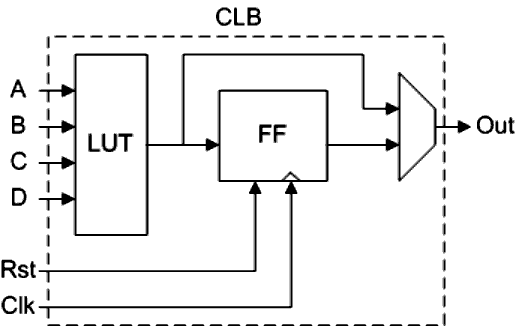
\includegraphics[scale=1.0]{FpgaCellExample.png}  
	\caption{Упрощённая схема логического блока FPGA}
	\label{fig:FpgaCellExample}
\end{figure}
 
В последние годы производители начали переходить на таблицы истинности с большим числом входов, что позволяет задействовать меньшее число логических блоков для типичных приложений.

Логический блок имеет таблицу истинности на 4 входа и вход синхронизации (\foreignlanguage{english}{clock}). Выход блока только один, это может быть регистровая или нерегистровая выходная таблица истинности. Поскольку сигналы синхронизации в коммерческих ППВМ (а часто и другие сигналы, распараллеливающиеся на большое количество входов — \foreignlanguage{english}{high-fanout signals}) трассируются особым образом специальными трассировочными цепями, управление этими сигналами делается отдельно.

Для приведённого примера архитектуры расположение контактов логического блока показано на рисунке~\ref{fig:FpgaLogicBlockPins}~\cite{Wiki_FPGA}

\begin{figure}[ht]
	\centering
	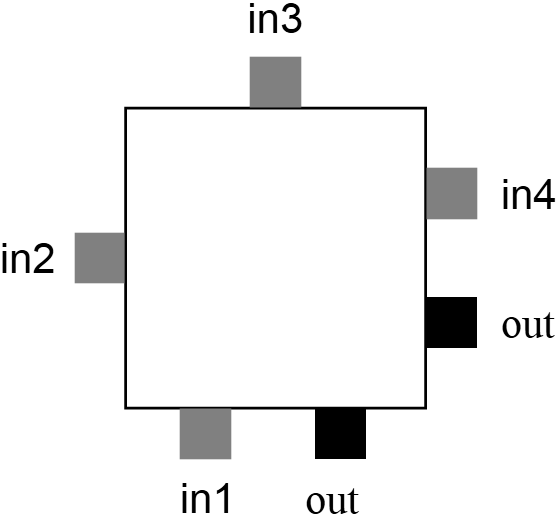
\includegraphics[scale=0.75]{FpgaLogicBlockPins.png}  
	\caption{Расположение контактов логического блока FPGA}
	\label{fig:FpgaLogicBlockPins}
\end{figure}

Входы расположены на отдельных сторонах логического блока, выходной контакт может трассироваться в двух каналах: либо справа от блока, либо снизу. Выходные контакты каждого логического блока могут соединяться с трассировочными сегментами в смежных каналах. Аналогично, контактная площадка блока ввода-вывода (pad) может соединяться с трассировочным элементом в любом смежном канале. Например, верхняя контактная площадка чипа может соединяться с любым из W проводников (где W - ширина канала) в горизонтальном канале, расположенном непосредственно под ним~\cite{Wiki_FPGA}.

Как правило, трассировка ППВМ несегментирована, то есть каждый сегмент проводника соединяет только один логический блок с переключательным блоком. Из-за огибания программируемых переключателей в переключательном блоке трассировка получается более длинной. Для увеличения скорости внутрисистемных соединений, в некоторых архитектурах ППВМ используются более длинные трассировочные соединения между логическими блоками~\cite{Wiki_FPGA}.

\begin{figure}[ht]
	\centering
	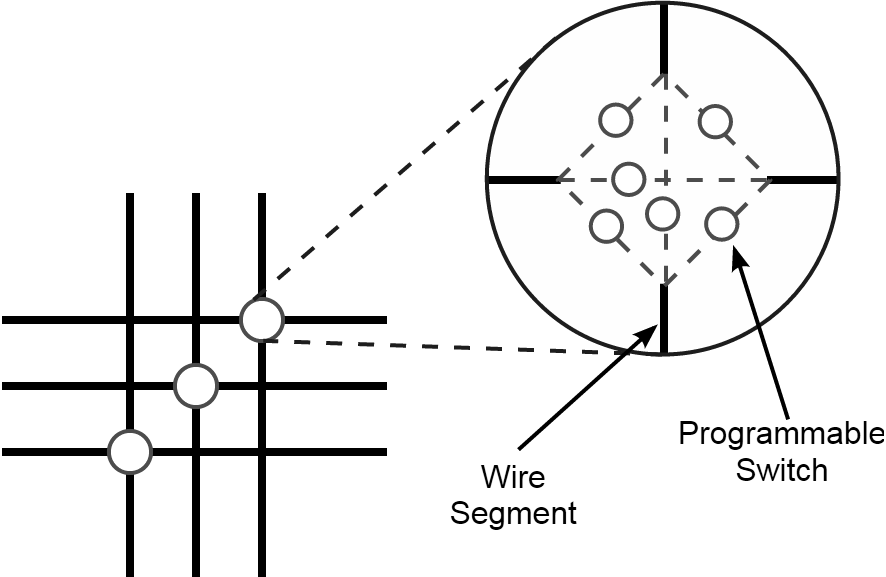
\includegraphics[scale=0.6]{FpgaSwitchBox.png}  
	\caption{Топология переключательного блока FPGA}
	\label{fig:FpgaSwitchBox}
\end{figure}

В месте пересечения вертикальных и горизонтальных каналов создаются переключательные блоки. При такой архитектуре для каждого проводника, входящего в переключательный блок, существуют три программируемых переключателя, которые позволяют ему подключаться к трём другим проводникам в смежных сегментах канала. Модель или топология выключателей, используемая в этой архитектуре, является планарной или доменной топологией переключательных блоков. В этой топологии проводник трассы номер один подключается только к проводнику трассы номер один в смежных каналах, проводник трассы номер 2 подключается только к проводникам трассы номер 2 и так далее. На рисунке~\ref{fig:FpgaSwitchBox} показаны соединения в переключательном блоке~\cite{Wiki_FPGA}.

% **************************************************
\subsection{Отладочная плата \boardname{}}
\boardname{}~--- это отладочная плата которая подходит как для обучения обучения, так и для разработки и тестирования систем на базе FPGA. Главный элемент данной платы~--- это FPGA-чип EP4CE115, который имеет более 100 тысяч логических элементов и является топовым внутри серии Cyclone~IV. Данный чип имеет следующие характеристики:
\begin{itemize}
	\item 114 480 логических элементов;
	\item 3 888 Кбит встроенной памяти;
	\item 266 встроенных умножителей разрядностью 18 x 18 бит;
	\item 4 блока ФАПЧ общего назначения.
	\item 528 пользовательских цифровых входов/выходов.
\end{itemize}

Отличительными особенностями платы являются:
\begin{itemize}
	\item 50 МГц тактовый генератор, 2 разъёма SMA для входа/выхода тактовой частоты;
	\item 2 МБайт SRAM, 2x64 МБайт SDRAM, 8 МБайт Flash, разъём для SD карт;
	\item 4 кнопки, 18 микропереключателей;
	\item 18 красных и 9 зелёных пользовательских светодиодов, ЖКИ 16x2;
	\item 24-разрядный аудио-кодек CD-качества с разъёмами линейного входа/выхода и микрофонного входа;
	\item VGA ЦАП (8-разрядный высокопроизводительный трёхканальный) с выходным VGA разъёмом;
	\item TV декодер (NTSC/PAL/SECAM) и разъём TV входа;
	\item 2 Gigabit Ethernet PHY с разъёмом RJ45;
	\item USB Host/ Slave контроллер с разъёмами USB type A и type B;
	\item Приёмопередатчик RS-232 с 9-контактным разъёмом, разъём PS/2 мыши/клавиатуры, ИК приёмник для пульта ДУ;
	\item 40-контактный разъём расширения с диодной защитой. Разъём для подключения мезонинных модулей (HSMC).
\end{itemize}

Особенно стоит отметить возмжность приобретение данной платы по студенческой цене, которая ниже, чем розничная стоимость отдельного FPGA-чипа, который установлен на плате.

В комплект платы \boardname{} входят следующие компоненты:
\begin{itemize}
	\item Плата DE2-115;
	\item USB кабель для программирования и управления FPGA;
	\item Системный CD, содержащий документацию на DE2-115 и материалы технической поддержки разработок;
	\item Комплект CD, содержащий ознакомительные версии ПО Altera’s Quartus II Web Edition и Nios II Embedded Design Suit;
	\item Пакет с 6 резиновыми (силиконовыми) колпачками для стоек платы DE2-115;
	\item Прозрачная пластмассовая защитная пластина для платы;
	\item 12 В сетевой источник питания;
	\item Пульт дистанционного управления.
\end{itemize}

Изображения платы с обеих сторон и расположение на ней компонентов показаны на рисунке~\ref{fig:FpgaBoard}.

\begin{figure}[ht]
\centering
  \begin{subfigure}[b]{1\textwidth} 
    \centering
    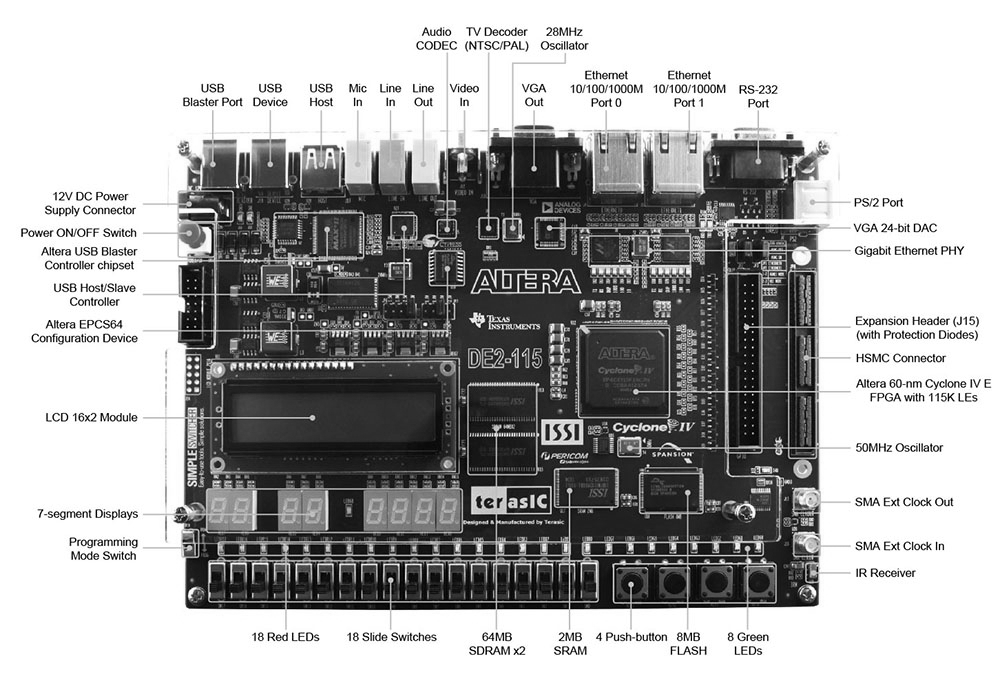
\includegraphics[scale=0.45]{FpgaBoardTop.jpg}  
    \caption{}
  \end{subfigure}
  \begin{subfigure}[b]{1\textwidth} 
    \centering
    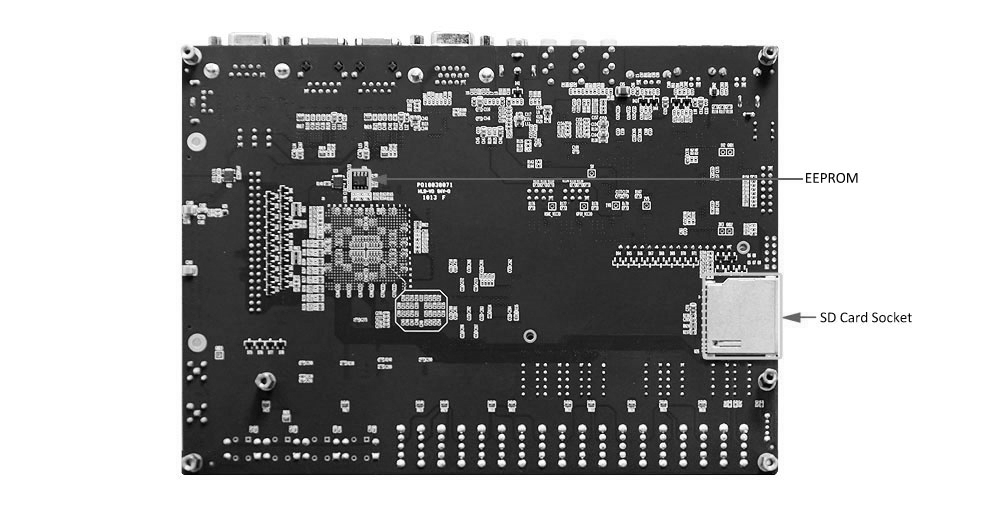
\includegraphics[scale=0.45]{FpgaBoardBottom.jpg}  
    \caption{}
  \end{subfigure}
  \caption{ Изображение платы \boardname{} и расположение на ней компонентов:
			а "--- с задней стороны;
			б "--- с передней стороны.}
  \label{fig:FpgaBoard}
\end{figure}

\section{Проектирование прототипа}
В этом разделе будут описаны некоторые этапы проектирования прототипа акустической камеры. В результате исследования теоретических материалов и проведения некоторых экспериментов была разработана структурная схема проектируемого устройства, которая показана на рисунке~\ref{fig:MainStructural}. Дальнейшее проектирование производилось в соответствии с данной схемой.

\begin{figure}[ht]
	\centering
	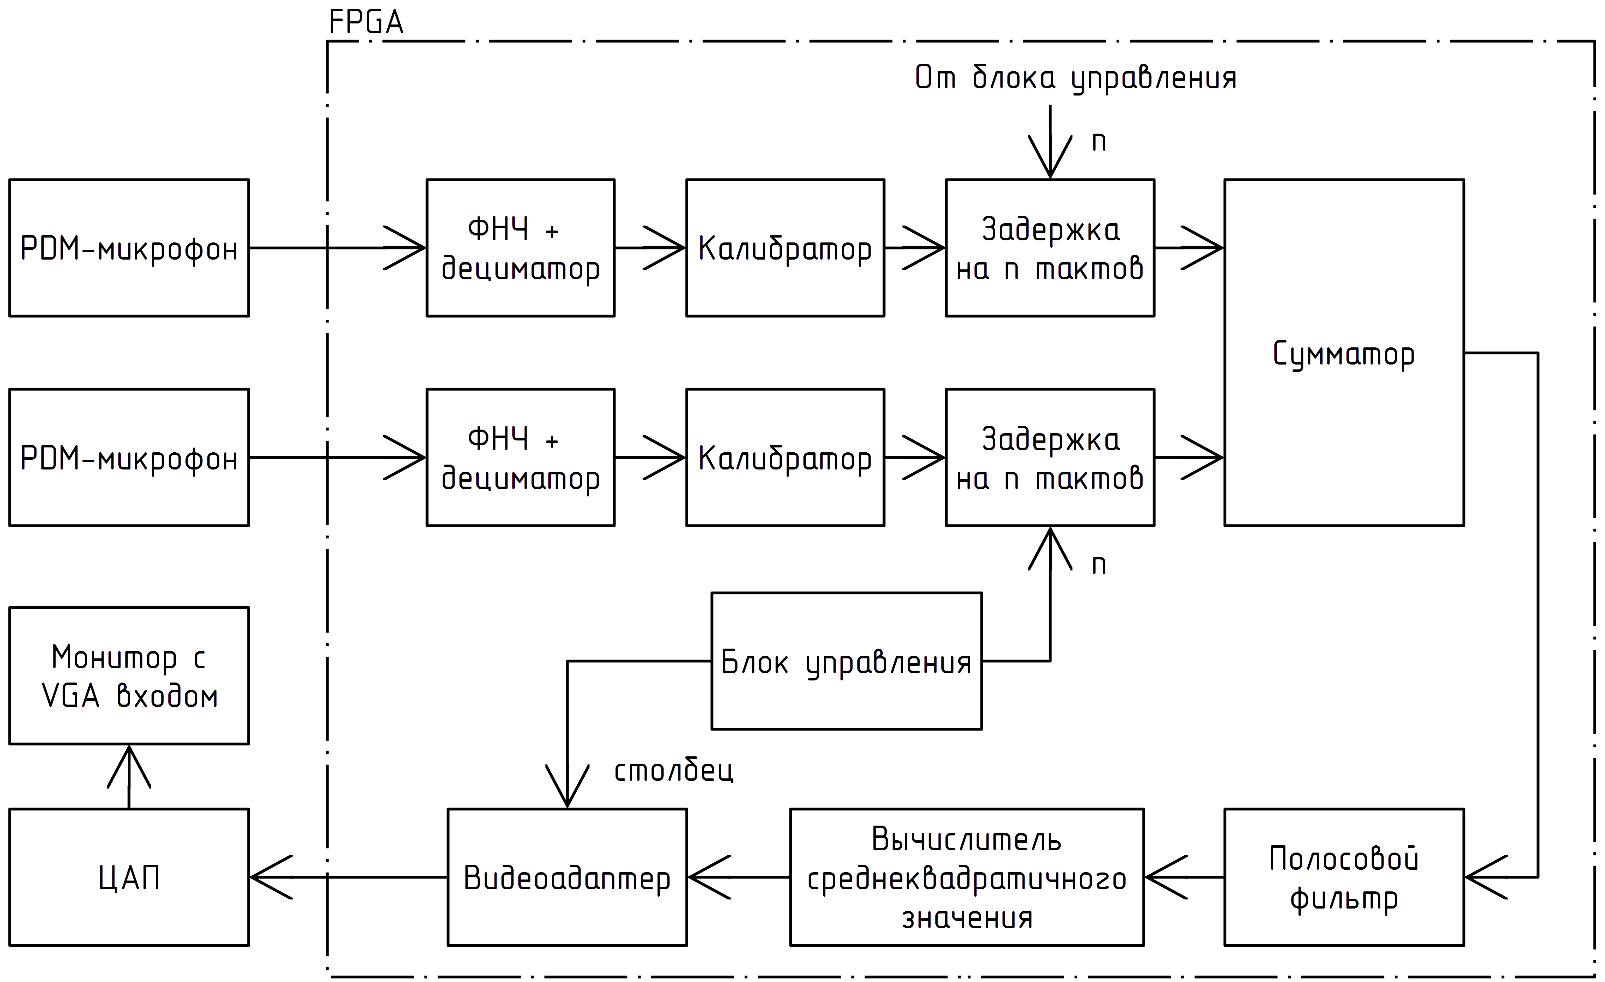
\includegraphics[scale=0.55]{MainStructural.png}  
	\caption{Структурная схема проектируемого устройства}
	\label{fig:MainStructural}
\end{figure}

% **************************************************
\subsection{Выбор параметров микрофонной решётки}
\label{section:MicArrayCalculations}
В виду сложности обработки данных с двумерной микрофонной решётки, в проекте решено применить одномерную микрофонную решётку. Единственным параметром характеризующим её конфигурацию является расстояние между микрофонами, которое необходимо рассчитать.

Уровень выходного сигнала полученного после суммирования отдельных сигналов со всех элементов линейной микрофонной решётки для определённой частоты можно вычислить по формуле~\cite{LabBookPages}:
\begin{equation}
	A = 20\lg{\left(\frac{1}{N}\sum_{i=0}^{N-1}e^{\frac{j2\pi{}fil\sin{\theta}}{c}}\right)}
\end{equation}
\begin{explanation}
	где &$A$& выходной сигнал, дБ; \\
	&$N$& количество датчиков микрофонной решётки; \\
	&$f$& частота входного сигнала, Гц; \\
	&$l$& расстояние между датчиками, м; \\
	&$c$& скорость звука, м/с; \\
	&$\theta$& угол падения звуковой волны на плоскость микрофонной решётки.
\end{explanation}

Построим зависимость уровня сигнала от $f$ и от $\theta$ при разных $N$ и $l$~\cite{LabBookPages} (см. рисунок~\ref{fig:BeamformerPatterns}). Для дальнейшего проектирования выберем решётку с параметрами $l = 0,04~\text{м}$ и $N = 15$. Выбор обусловлен следующими причинами:
\begin{itemize}
	\item Число микрофонов приемлемо для построения решётки в домашних условиях;
	\item Расстояние между микрофонами не слишком велико, следовательно общая длинна решётки останется приемлемой;
	\item Подавление сигнала вне диапазона чувствительности является вполне достаточным;
	\item Рабочий диапазон частот 3~--~6~кГц близок к спектру человеческого голоса;
\end{itemize}

Для удобства проектирования печатной платы, число микрофонов выберем равным 16.

\begin{figure}[ht]
	\centering
	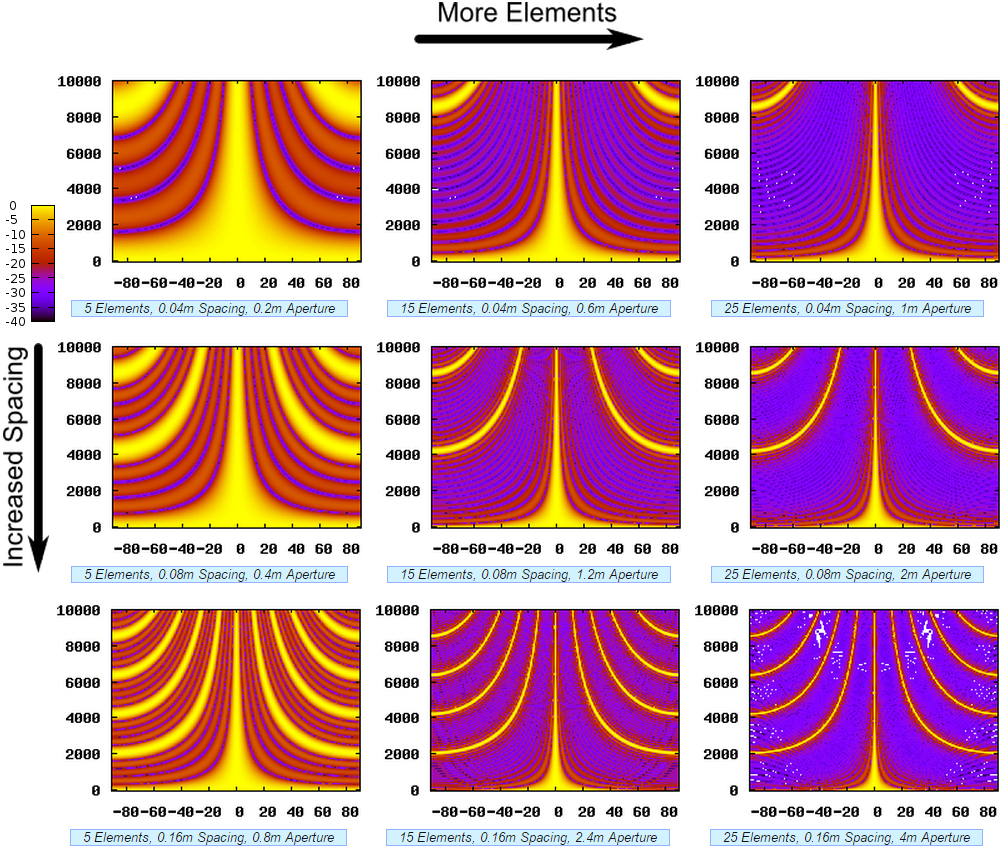
\includegraphics[scale=0.6]{BeamformerPatterns.png}  
	\caption{Зависимость уровня выходного сигнала бимформера от угла падения звуковой волны и от частоты сигнала при различном количестве датчиков и разном расстоянии между ними}
	\label{fig:BeamformerPatterns}
\end{figure}

% **************************************************
\subsection{Разработка печатных плат для микрофонной решётки}
\label{section:PcbBuilding}
Микрофоны применяемые в данном проекте выпускаются только в корпусах для поверхностного монтажа, поэтому для соединения каждого из них с блоком обработки данных, необходимо разработать и создать печатную плату. Учитывая, что микрофонная решётка состоит из 16-ти микрофонов, которые размещены на расстоянии 40 мм друг от друга, общая длинна платы равнялась бы не менее 0,6 метрам. Цельный кусок фольгированного текстолита такого размера достаточно трудно найти. Поэтому плата была разбита на 4 части по 160 мм каждая. Также была разработана плата-соединитель для подключения всех остальных плат к плате \boardname{}. 

В качестве программного обеспечения для проектирования платы была выбрана программа Sprint-Layout 6.0. Такой выбор обоснован простотой этой программы, а также простотой разрабатываемой платы, которая не требует каких либо особых возможностей от среды проектирования.

При проектировании рисунка печатной платы было соблюдено рассчитанное ранее расстояние между микрофонами в 40 мм. На края платы были добавлены контактные площадки для возможности её соединения с соседними платами. Стоит также отметить, что плата-соединитель, размещённая между двумя обычными платами увеличивает расстояние межу микрофонами. Поэтому, на плату были добавлены дополнительные контактные площадки на некотором расстоянии от края. Это позволит срезать часть платы со стороны прилегающей к плате-соединителю, не лишившись при этом контактных площадок.

В виду невозможности развести для данного проекта одностороннюю печатную плату без перемычек, шины данных микрофонов были выведены на специальные площадки и соединены с платой-соединителем с помощью проводов.

В результате разработки получилась печатная плата, показанная на рисунке~\ref{fig:Pcb4Mic}. Плата-соеденитель представлена на рисунке~\ref{fig:PcbConnector}

\begin{figure}[ht]
	\centering
	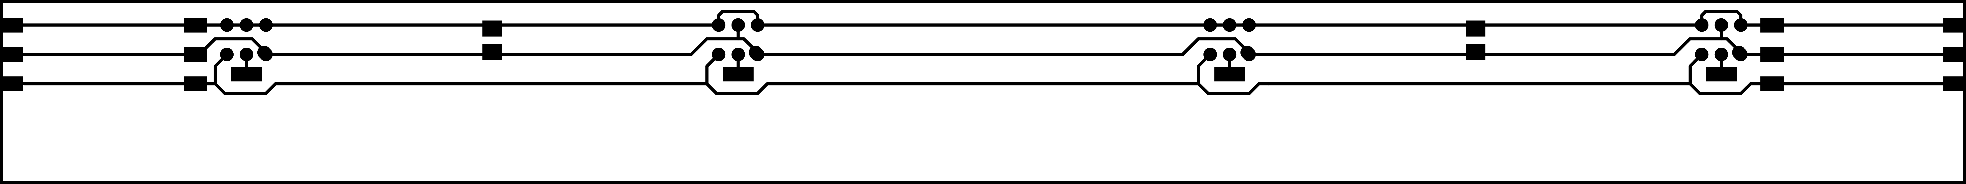
\includegraphics[scale=0.95]{Pcb4Mic.png}  
	\caption{Печатная плата для четырёх микрофонов}
	\label{fig:Pcb4Mic}
\end{figure}

\begin{figure}[ht]
	\centering
	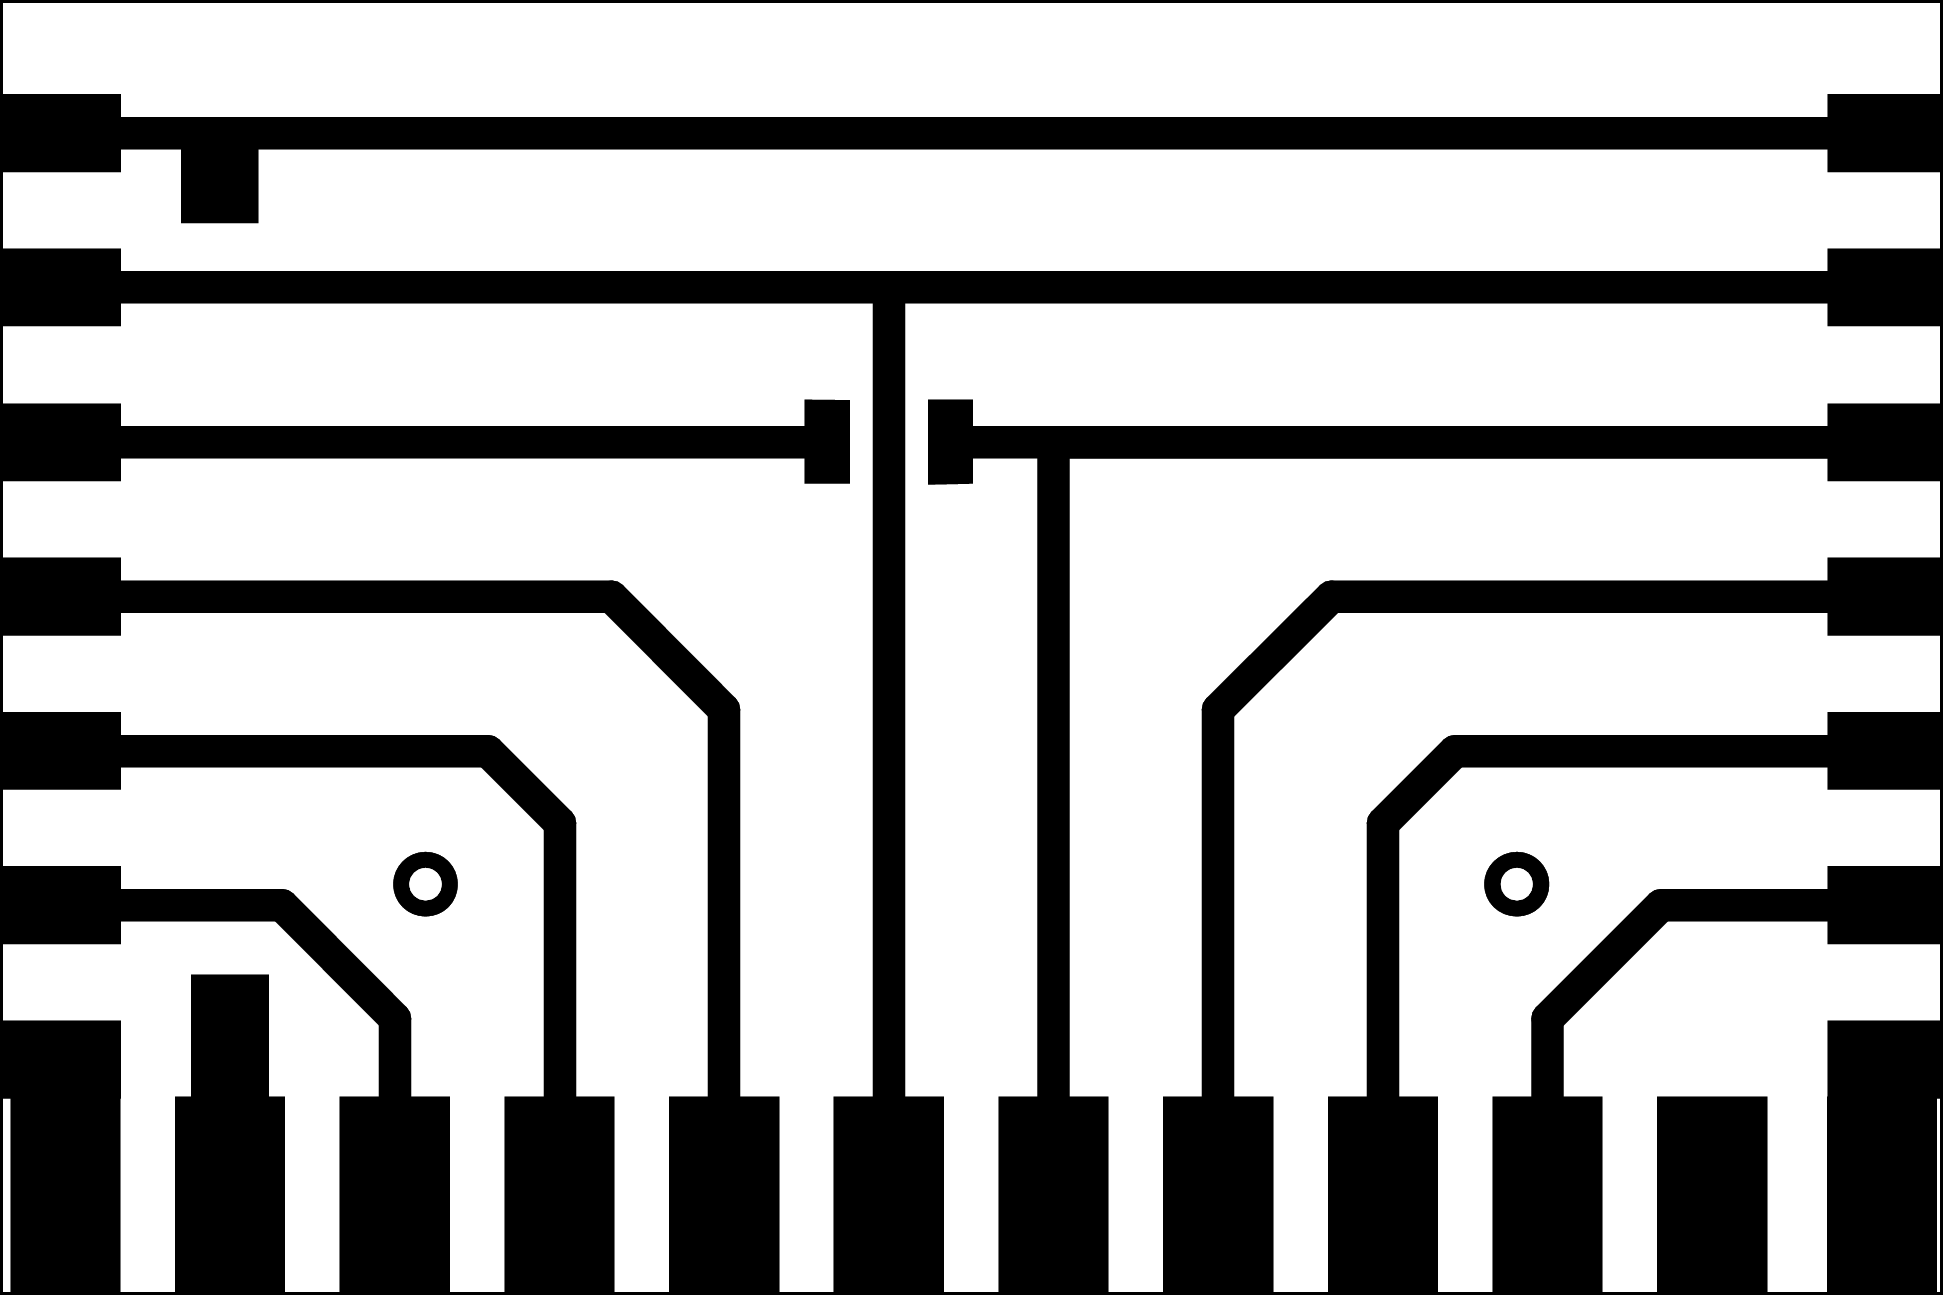
\includegraphics[scale=0.95]{PcbConnector.png}  
	\caption{Печатная плата-соединитель}
	\label{fig:PcbConnector}
\end{figure}

По разработанным рисункам были произведены лазерно-утюжным методом четыре обычных платы и одна плата-соединитель. Затем на них были припаяны компоненты, а сами платы соединены между собой каплями припоя. Вся система была закреплена на деревянной рейке длинной 640 мм с помощью нейлоновых стяжек.

\subsubsection{Тестирование печатной платы. }
Для того, чтобы проверить правильность разработки печатной платы, а также надёжность пайки компонентов, микрофонная решётка была подключена к плате \boardname{} и с помощью заранее разработанной прошивки с каждого микрофона были сняты данные, при воспроизведении звукового сигнала частотой 1 кГц на некотором расстоянии от решётки. Данные были записаны в статическую память, расположенную на плате и переданы на ПК через JTAG отладчик. Затем, с помощью скрипта на языке Python полученные данные были преобразованы в удобную для обработки форму, после чего были обработаны скриптом на языке MATLAB для получения спектра сигнала. Результат такой обработки для одного из микрофонов показан на рисунке~\ref{fig:PdmMicSpectrum}.

\begin{figure}[ht]
	\centering
	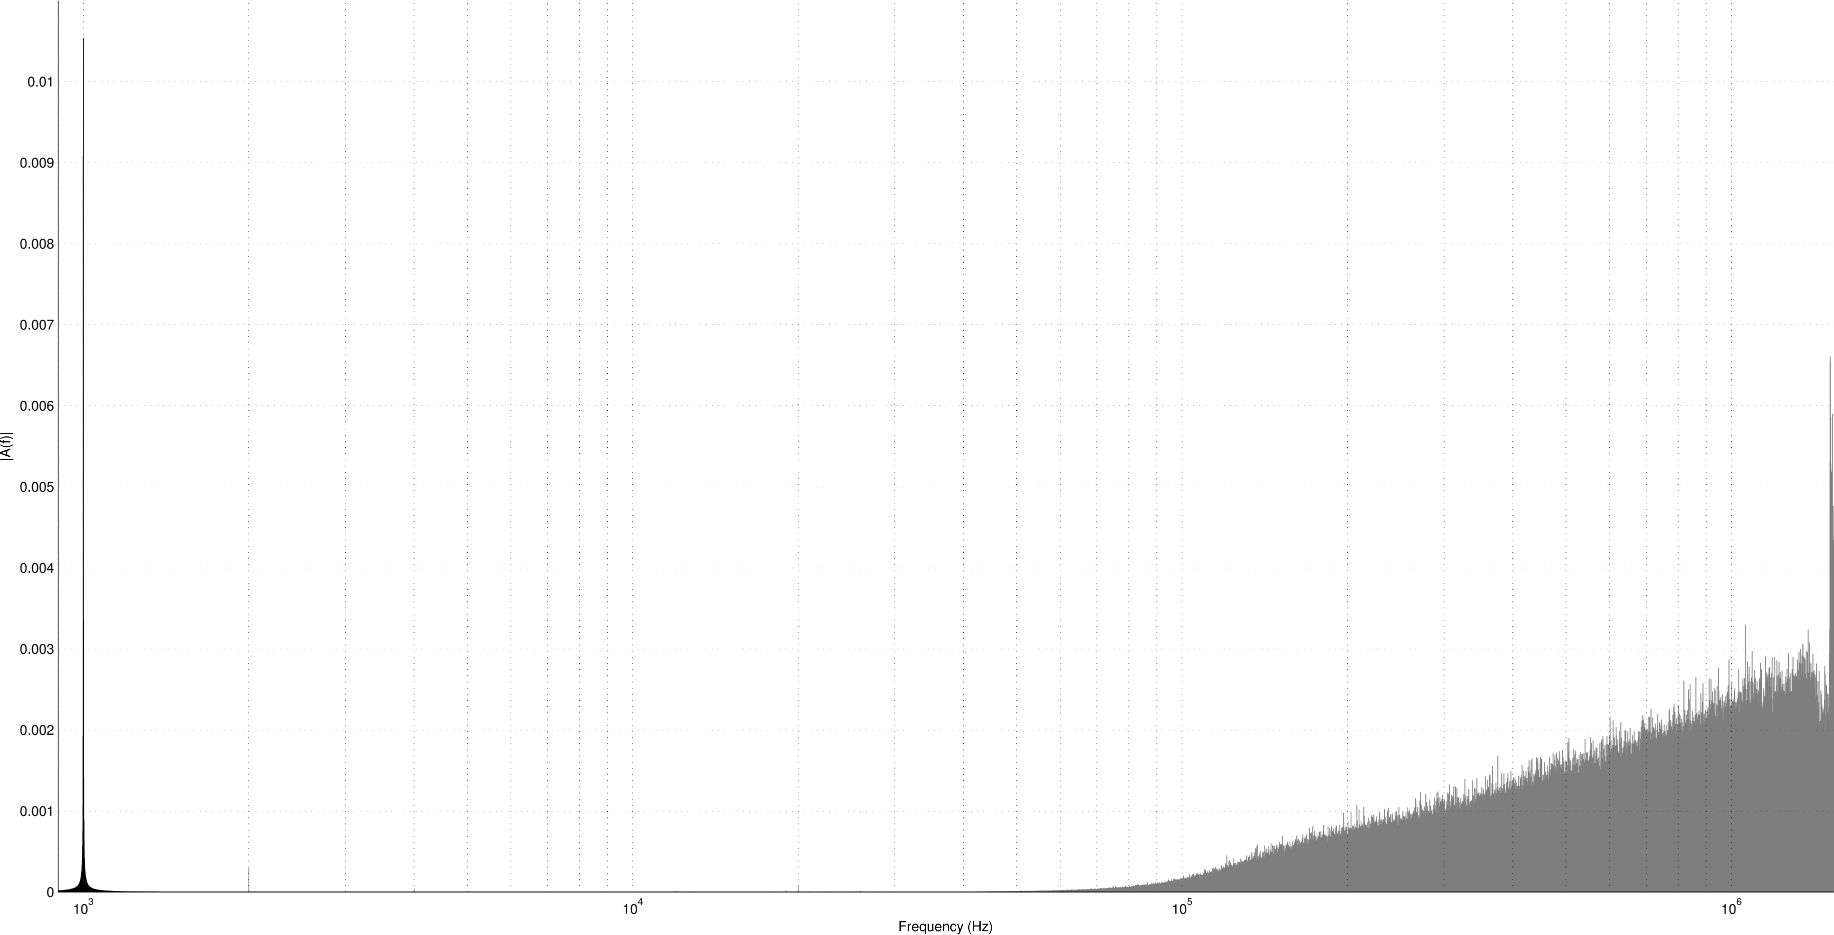
\includegraphics[scale=0.33]{PdmMicSpectrum.png}  
	\caption{Спектр сигнала, полученного с микрофона \micname{}}
	\label{fig:PdmMicSpectrum}
\end{figure}

% **************************************************
\subsection{Разработка многоканального фильтра нижних частот}
\label{section:LowPassFilterBuilding}
 Чтобы снизить стоимость разработки проекта, в качестве датчиков в микрофонной решётке целесообразно применить цифровые PDM-микрофоны. Для того, чтобы произвести дальнейшую обработку сигналов полученных с этих микрофонов, необходимо для начала преобразовать их из формата PDM (см. раздел~\ref{section:pdm}) в формат PCM (импульсно-кодовая модуляция), в котором каждый отсчёт сигнала представлен двоичным числом определённой разрядности. Чтобы понять, как это сделать, необходимо взглянуть на спектр PDM-сигнала, полученного с микрофона \micname{}. Для получения спектра , который изображён на рисунке~\ref{fig:PdmMicSpectrum}. Из рисунка видно, что желаемый сигнал уже является частью спектра исходного сигнала, но помимо него присутствует ещё довольно большое количество шума. Однако, этот шум практически полностью сосредоточен в верхней части спектра. Следовательно, чтобы выделить желаемый сигнал, достаточно всего-лишь пропустить исходный сигнал через фильтр нижних частот (в дальнейшем ФНЧ). Т. к. после фильтрации полученный сигнал больше не будет содержать высокочастотных компонентов, то целесообразно понизить и без того завышенную частоту дискретизации этого сигнала с помощью децимации. Как будет видно в дальнейшем, децимация позволит оптимизировать вычисления производимые фильтром.

\subsubsection{Формулировка требований к ФНЧ. }
Исходя из задачи решаемой проектируемым фильтром, к нему были предъявлены следующие требования:
\begin{itemize}
	\item Способность обеспечивать подавление шума вне полосы пропускания на таком уровне, чтобы данный шум после децимации не сильно ухудшил характеристики полезного сигнала. Чтобы определится со степенью подавления, откроем документацию на микрон \micname. Можно заметить, что отношение сигнал-шум для этого микрофона составляет 61 дБ. Целесообразно выбрать степень подавления таким образом, чтобы с одной стороны не сильно ухудшить этот параметр, а с другой стороны не сделать реализацию фильтра слишком затратной. Поэтому степень подавления была выбрана равной величине в $-100$ дБ.
	\item Для того чтобы не вносить частотные искажения в полезный сигнал, необходимо обеспечить ровную АЧХ во всей полосе пропускания фильтра.
	\item За верхнюю границу полосы пропускания фильтра примем верхнюю границу слышимого человеком диапазона~--- 20~кГц.
	\item Для дальнейшей оптимизации фильтра необходимо выбрать его коэффициент децимации равным степени двойки. Также, согласно теореме Котельникова, этот коэффициент должен снижать первичную частоту дискретизации до уровня как минимум в два раза большего верхней границы фильтра. Исходя из этого выберем коэффициент децимации равным 64.
\end{itemize}

\subsubsection{Выбор типа ФНЧ. }
Согласно разделу~\ref{section:DigitalFilters}, цифровые фильтры бывают двух основных типов: КИХ (раздел~\ref{section:FIR}) и БИХ (раздел~\ref{section:IIR}). Несмотря на некоторые преимущества БИХ фильтров перед КИХ фильтрам, а именно, наличие лучших характеристики при меньшем порядке, а также использование меньшего операций при реализации на цифровых сигнальных процессорах, в данном проекте было решено использовать КИХ-фильтр.

Одной из причин выбора именно КИХ-фильтра является следующий факт. Если взглянуть на структурную схему фильтра (рисунок~\ref{fig:FirStructure}, то можно заметить, что с входным сигналом производится множество операций умножения. А в виду того, что в данном проекте используется FPGA, то целесообразно попытаться избавиться от этой операции, т. к. это позволит освободить дополнительное место на кристалле, занимаемое логикой умножителя. Теперь, вспомним, что мы имеем дело с однобитным сигналом, для которого операция умножения на некую константу $b$ по сути представляет собой взятие этой константы либо со знаком $+$, либо со знаком $-$. Таким образом, полноценный умножитель не потребуется. БИХ-фильтр из-за наличия обратной связи не позволяет выполнить такую оптимизацию.

Абсолютная стабильность и простота реализации также делают КИХ-фильтр очень заманчивым решением.

\subsubsection{Расчет коэффициентов фильтра. }
Для расчётов фильтр была использована утилита FDATool, которая входит в программный пакет MATLAB. Исходя требований к фильтру были рассчитаны его коэффициенты, а затем произведена их квантизация для возможности использования арифметики с фиксированной точкой, при реализации фильтра на FPGA. Результирующий фильтр имеет 18-ти битные коэффициенты, 4095-й порядок и амплитудно-частотную характеристику показанную на рисунке~\ref{fig:LowPassFilterMagnitude}
\begin{figure}[ht]
	\centering
	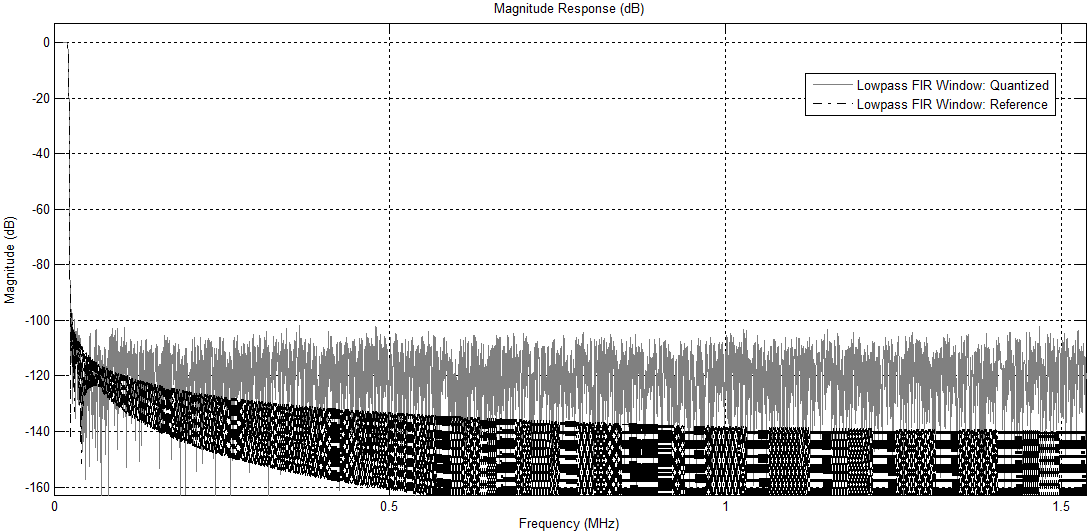
\includegraphics[scale=0.56]{LowPassFilterMagnitude.png}  
	\caption{АЧХ рассчитанного фильтра при использовании коэффициентов с плавающей (серая сплошная линия) и фиксированной (чёрная пунктирная линия) точкой}
	\label{fig:LowPassFilterMagnitude}
\end{figure}

\subsubsection{Реализация фильтра с учётом особенностей FPGA и решаемой фильтром задачи. }
В FPGA серии Cyclone VI фирмы Altera есть встроенный конфигурируемые блоки памяти объёмом 9 килобит каждый. С учётом того, что разрядность коэффициентов фильтра была рассчитана равной 18-ти битам, в каждом блоке поместится 512 коэффициентов. Таким образом, для хранения всех коэффициентов фильтра 4095-го порядка понадобится 8 блоков памяти. Причём, каждый блок можно разместить внутри отдельного вычислительного блока, что обеспечить параллельность вычислений. Структуру каждого вычислительного блока упрощённо так, как показано на рисунке~\ref{fig:LowPassFilterStructure}.
\begin{figure}[ht]
	\centering
	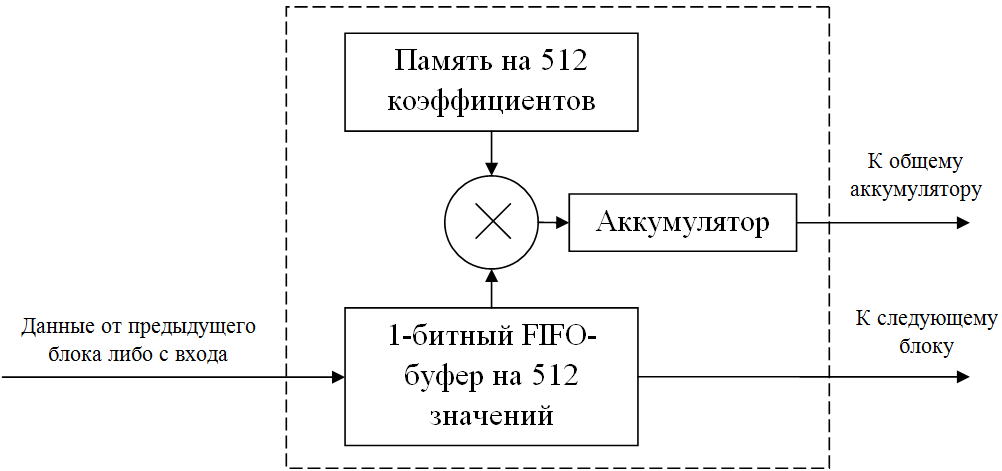
\includegraphics[scale=0.6]{LowPassFilterStructure.png}  
	\caption{Упрощённая структура вычислительного блока КИХ-фильтра, реализованного на FPGA}
	\label{fig:LowPassFilterStructure}
\end{figure}

Микрофон \micname{} тактируется частотой около 3 МГц. Если учесть, что с такой частотой нужно вычислять 512 коэффициентов, то частота каждой операции будет равна 1,5 ГГц. Недорогие ПЛИС не способны работать на такой частоте.
 
Оптимизируем вычисления, имея в виду, что после фильтра производится децимация сигнала с коэффициентом 64. Это означает, что имеет смысл вычислять только каждый 64-й отсчёт. Поэтому, мы можем растянуть во времени вычисление нужных отсчётов, отбросив при этом ненужные. Тогда частота выполнения каждой операции фильтра станет равна всего $3 \cdot{} 512 / 64 = 24$ МГц. Такая частота является вполне приемлемой для используемого в проекте FPGA-чипа.

\subsubsection{Вывод. }
В результате расчётов и анализа возможных оптимизаций, удалось спроектировать фильтр 4095-го порядка, состоящий из восьми вычислительных блоков и работающий на частоте 24 МГц, что всего в 4 раза превосходит частоту дискретизации входного сигнала.

% **************************************************
\subsection{Реализация \dands{} бимформера}
\label{section:BeamformerBuilding}
Согласно разделу~\ref{section:DelayAndSumBeamforming} \dands{} бимформер состоит из сумматора и элементов с контролируемой задержкой. Т. к. реализация сумматора на FPGA является тривиальной, то она не представляет интереса не будет рассмотрена в этой работе.

Рассмотрим способы реализации элемента с контролируемой задержкой.

\subsubsection{Задержка на основе регистров. }
Самым простым решением поставленной задачи является задержка на основе регистров. Её схема показана на рисунке~\ref{fig:RegisterDelay}. Схема состоит из мультиплексора и регистров (или групп регистров в случае многобитного сигнала), соединённых последовательно. Каждый из этих регистров выполняет задержку на один такт. Таким образом, выбрав нужный сигнал с помощью мультиплексора, можно получить сигнал с задержкой на нужное число тактов.
\begin{figure}[ht]
	\centering
	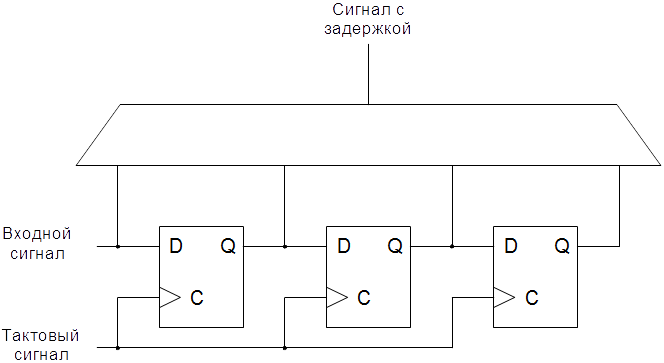
\includegraphics[scale=0.9]{RegisterDelay.png}  
	\caption{Задержка на основе регистров}
	\label{fig:RegisterDelay}
\end{figure}

Данный способ задержки сигнала был опробован при реализации данного проекта. Однако, он оказался не эффективен, т. к. потреблял слишком много ресурсов FPGA-чипа. В результате было решено от него отказаться.

\subsubsection{Задержка на основе блочной памяти. }
Другой подход можно применить при реализации задержки на основе блочной двухпортовой памяти. Такая память показана на рисунке~\ref{fig:MemoryDelay}. Она имеет две шины адреса: А и Б, а также две шины данных: одна для записи, другая для чтения. Входной сигнала поступает на шину А. При этом адрес на шине адреса А меняется на каждом такте. Таким образом, память последовательно заполняется входными данными. При переполнении памяти запись начинается с нулевого адреса, а старые данные стираются. С шины данных Б происходит считывание задержанного сигнала. При этом величина задержки определяется разница адресов А и Б, а её максимальное значение равно ёмкости памяти.

Такой способ организации задержки оказался гораздо экономичнее предыдущего, т. к. при его реализации используются не логические элементы, а блочная память встроенная в FPGA.
\begin{figure}[ht]
	\centering
	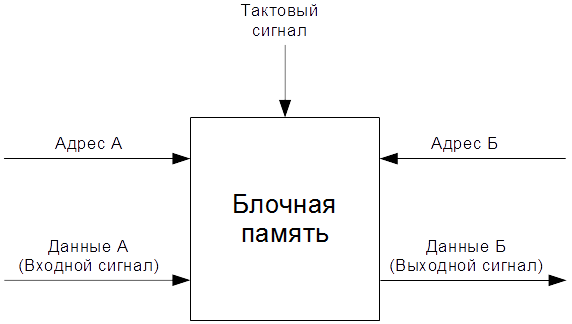
\includegraphics[scale=0.9]{MemoryDelay.png}  
	\caption{Задержка на основе блочной двухпортовой памяти}
	\label{fig:MemoryDelay}
\end{figure}


% **************************************************
\subsection{Разработка полосового фильтра}
\label{section:BandPassFilterBuilding}
Если взглянуть на рисунок~\ref{fig:BeamformerPatterns}, то можно заметить, что \dands{} бимформер имеет плохую пространственную избирательность в области низких частот. А в области высоких частот проявляется эффект пространственного алиасинга, в результате на диаграмме направленности появляются так называемые ложные лепестки (англ. \foreignlanguage{english}{grating lobes}~--- раздражающие лепестки). Чтобы избавится от этих нежелательных эффектов, необходимо чтобы бимформер работал только в определённом диапазоне частот. Для этого понадобится разработать полосовой фильтр.

Зададимся полосой пропускания фильтра 3~--~6 кГц. Степень подавления вне полосы пропускания выберем 80 Дб. Данный фильтр лучше всего реализовать в виде БИХ структуры для экономии ресурсов FPGA. Запустим утилиту FDATool из программного пакета MATLAB и произведём расчёт фильтра согласно исходным данным. Полученный фильтр имеет 32-й порядок и амплитудно-частотную характеристику изображённую на рисунке~\ref{fig:BandPassFilterResponse}.
\begin{figure}[ht]
	\centering
	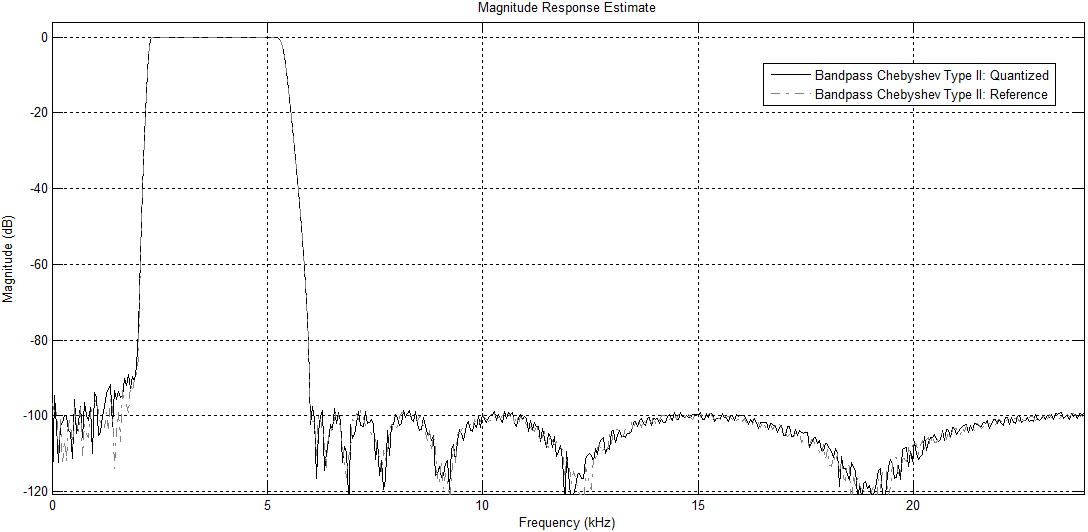
\includegraphics[scale=0.54]{BandPassFilterResponse.png}  
	\caption{Амплитудно-частотная характеристика рассчитанного полосового фильтра при использовании коэффициентов с плавающей (пунктирная серая линия) и фиксированной (чёрная сплошная линия) точкой}
	\label{fig:BandPassFilterResponse}
\end{figure}

В качестве формы БИХ фильтра была выбрана первая прямая форма (англ. \foreignlanguage{english}{Direct Form I Structure}). Такая форма не является самой оптимальной с точки зрения потребляемых ресурсов, однако она позволяет значительно снизить ошибку округления, которая присуща реализации фильтра с использованием арифметики с фиксированной точкой~\cite{Xilinx_IIR}. Также, для снижения ошибки округления и повышения устойчивости фильтра его целесообразно разбить на секции второго порядка (англ. \foreignlanguage{english}{Second Order Section, SOS}). Структура секции второго порядка в первой прямой форме показана на рисунке~\ref{fig:SosStructure}
\begin{figure}[ht]
	\centering
	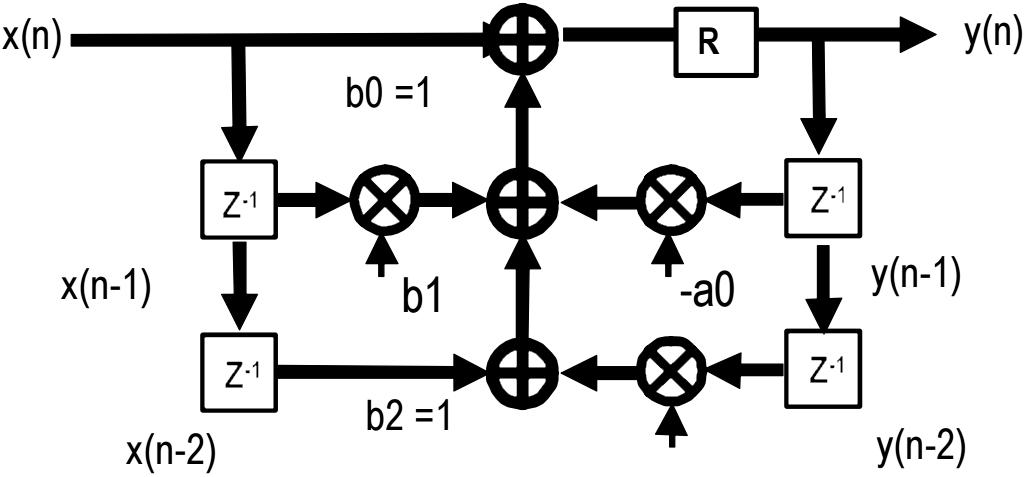
\includegraphics[scale=0.6]{SosStructure.png}  
	\caption{Секция второго порядка в первой прямой форме}
	\label{fig:SosStructure}
\end{figure}

После реализации на языке SystemVerilog данный фильтр был просимулирован в программе ModelSim. Переходная характеристика полученная в результате симуляции полностью совпадает с расчётной. Её вид представлена на рисунке~\ref{fig:BandPassFilterSim}. После, дизайн был скомпилирован и протестирован на плате \boardname{}, а правильность его работы была оценена качественным образом. 
\begin{figure}[ht]
	\centering
	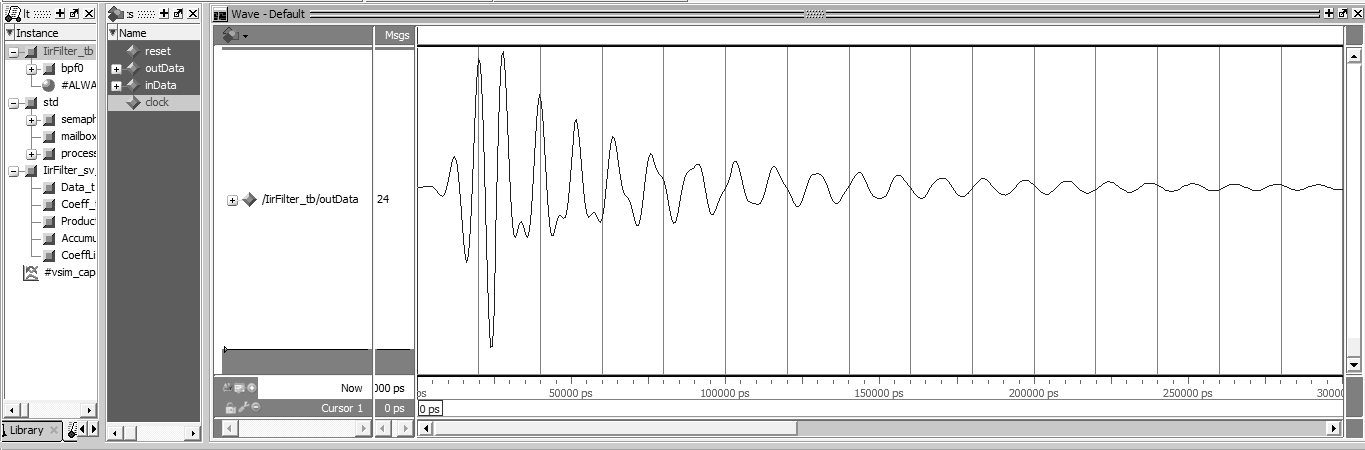
\includegraphics[scale=0.45]{BandPassFilterSim.png}  
	\caption{Переходная характеристика полученная в результате симуляции разработанного фильтра}
	\label{fig:BandPassFilterSim}
\end{figure}

% **************************************************
\subsection{Разработка простейшего видеоадаптера}
\label{section:VideoAdapterBuilding}
В требованиях к проекту указана необходимость отображать результат обработки сигналов на ЖК монитор разрешением 1024 x 768 пикселей. Т. к. на плате \boardname{} присутствуют только VGA-разъём и видео-ЦАП, то для осуществления вывода изображения на монитор придётся формировать сигналы вертикальной и горизонтальной синхронизации средствами FPGA. Также необходимо предусмотреть видео-память для хранения выводимого на дисплей изображения. Рассмотрим подходы к построению данного видеоадаптера.

Самым простым способом реализовать видеоадаптер является организация попиксельного вывода изображения из памяти на дисплей. Подсчитаем объём памяти необходимый для хранения видеоизображения. Яркость свечения каждого пикселя можно записать с помощью одного бита данных (активный и неактивный пиксель). Всего имеется $1024 \cdot{} 768 = 786 432$ пикселей. Таким образом, для хранения целого изображения понадобится 768 кбит. Учитывая, что в выбранном FPGA-чипе встроено 3,89 Мбит памяти, такой дизайн видеоадаптера  занял бы большую часть ресурсов чипа. Следовательно описанный подход не рационален.

\begin{figure}[ht]
	\centering
	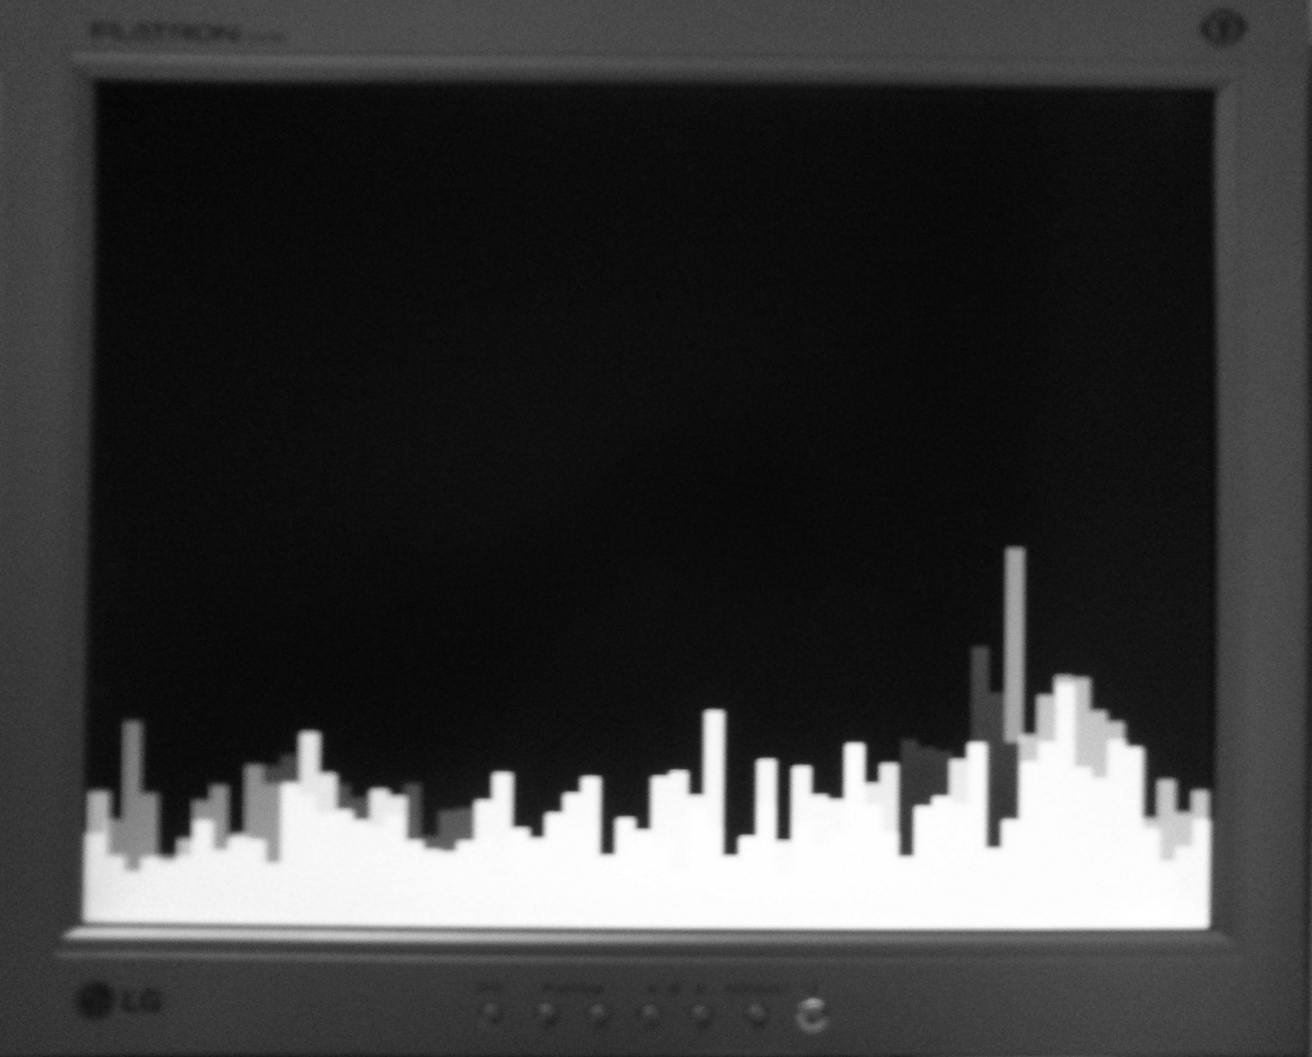
\includegraphics[scale=0.35]{VideoAdapterResult.jpg}  
	\caption{Изображение полученное на ЖК-мониторе с помощью разработанного видеоадаптера}
	\label{fig:VideoAdapterResult}
\end{figure}

Рассмотрим теперь альтернативный подход с учётом особенностей выводимого изображения. В качестве средства для индикации угла с которого пришёл звуковой сигнал определим набор из 64-х столбцов, заполняющих всю ширину экрана. Высота столбца будет будет показывать амплитуду сигнала, а номер столбца~--- угол с которого этот сигнал пришёл (столбец 0~--- $-90^{\circ}$, столбец 63~--- $90^{\circ}$). При этом отпадает необходимость хранить в памяти всё изображение целиком. Цвет пикселя может быть определён исходя из координат этого пикселя и требуемой высоты столбца в зону которого этот пиксель попадает. Таким образом в памяти можно хранить только требуемые высоты столбцов, а её объём определяется исходя из количества градаций высоты столбца и количества столбцов. Для 768-ми градаций и 64-х столбцов этот объем составит всего 7,68 кбит, что ровно на два порядка меньше, чем в предыдущем подходе. В связи с этим именно такое решение было применено в данном проекте.

Результат работы спроектированного видеоадаптера можно увидеть на рисунке~\ref{fig:VideoAdapterResult}.

% **************************************************
\subsection{Результат разработки и решение возникших проблем}
\label{section:ResultAndProblems}
После разработки всех частей и объединения их в единую систему, были произведены испытания полученного устройства. Не смотря на то, что все части по отдельности работали без нареканий, работа устройства в целом оставляла желать лучшего. Главный недостаток заключался в низкой пространственной чувствительности. Т. е. несмотря на отличную чувствительность устройства к звуковым волнам из рабочего диапазона, определить положение источника звука по данным с экрана было хоть и возможно, но несколько затруднительно из-за слабой выраженности направленных свойств микрофонной решётки. Чтобы решить данную проблему было сделано несколько гипотез.

\subsubsection{Калибровка. }
Первая гипотеза состоит в следующем: если один или несколько микрофонов имеют чувствительность намного больше, чем большинство других в системе, то сигнал получаемый с более чувствительных микрофонов будет доминирующим в сумме и из-за всенаправленности отдельного микрофона снизится пространственная чувствительность всей системы.

Чтобы проверить эту гипотезу были произведены измерения чувствительности микрофонов. Для этого была разработана специальная прошивка для платы \boardname{} и написано несколько скриптов на языках TCL, Python и MATLAB, которые позволили записать синал одновременно с 16-ти микрофонов, передать полученные данные на ПК и произвести их анализ. Во время записи на микрофоны был подан звуковой сигнал частотой 100 Гц. Такая частота была выбрана после предварительных экспериментов, показавших, что звуковые волны более высоких частот отражаются от стен помещения и образуют стоячие волны, которые мешают проведению измерений. После записи данных и передачи их на ПК, с помощью пакета MATLAB были построены АЧХ для сигналов с каждого из микрофонов. Результат построения можно увидеть на рисунке~\ref{fig:CalibrationMagnitudeResponse}, из которого видно, что сигналы отличаются незначительно.

\begin{figure}[ht]
	\centering
	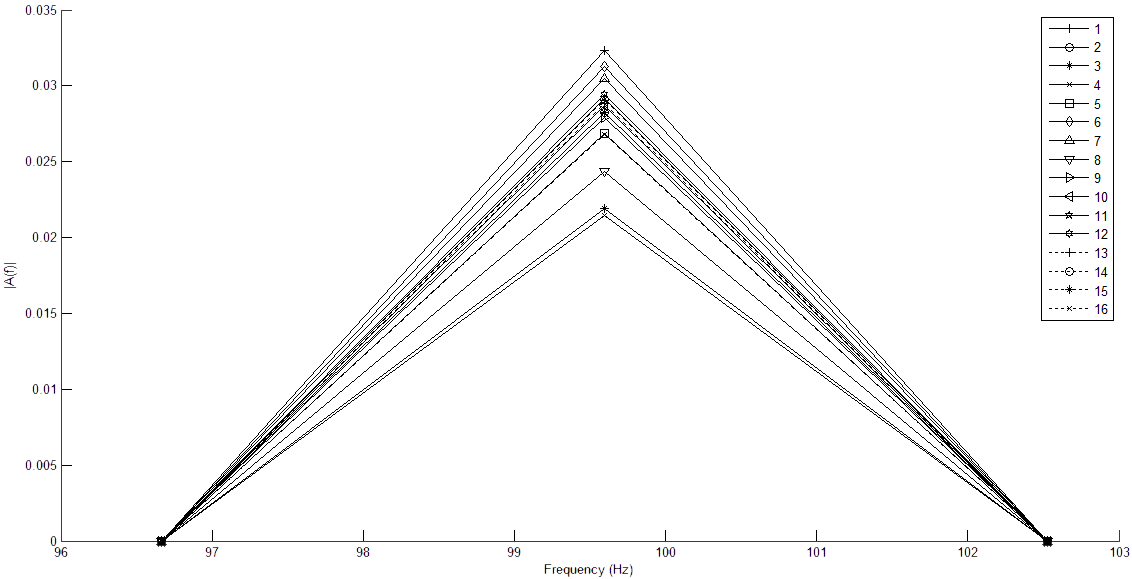
\includegraphics[scale=0.55]{CalibrationMagnitudeResponse.png}  
	\caption{}
	\label{fig:CalibrationMagnitudeResponse}
\end{figure}

Чтобы до конца проверить гипотезу, по данным о чувствительности микрофонов были получены масштабирующие коэффициенты, а в систему добавлен новый элемент~--- калибратор, который производит ослабление сигналов с микрофонов в соответствии с этими коэффициентами. После введения в систему калибратора, были снова проведены тесты пространственной чувствительности. Однако, каких либо заметных улучшений не наблюдалось и данная гипотеза была отвергнута.

\subsubsection{Фазировка. }
Другая выдвинутая гипотеза строится на предположении о том, что микрофоны могут быть не сфазированы из-за особенностей их производства. Работая в противофазе такие микрофоны выдавали бы сигналы не способные коррелировать, что могло бы обуславливать низкую пространственную чувствительность системы.

Для проверки данной гипотезы были взяты данные, полученные в процессе калибровки и по ним построены фазовые характеристики сигналов. Результат этого построения представлен на рисунке~\ref{fig:CalibrationPhaseResponse}. Из этих характеристик видно, что сдвига фаз в $180^{\circ}$ между сигналами не наблюдается. Таким образом, данная гипотеза была также отвергнута.

\begin{figure}[ht]
	\centering
	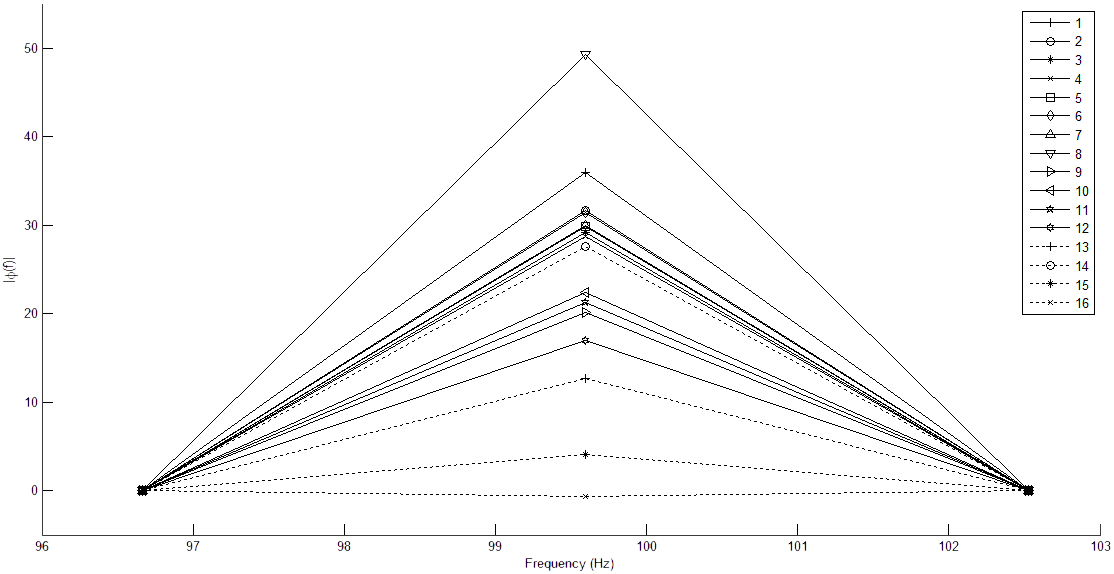
\includegraphics[scale=0.55]{CalibrationPhaseResponse.png}  
	\caption{}
	\label{fig:CalibrationPhaseResponse}
\end{figure}

\subsubsection{Случайные сдвиги фаз. }
На основе данных полученных при проверке предыдущей гипотезы, возникла третья гипотеза. Если взглянуть ещё раз на рисунок~\ref{fig:CalibrationPhaseResponse}, то можно заметить наличие случайных сдвигов фаз между сигналами хоть и меньших $180^{\circ}$, но всё же значительных и потенциально способных привести к наблюдаемым негативным эффектам. Причина этих сдвигов на данный момент не ясна, и может заключаться в неправильно выполненных измерениях. Тогда данную гипотезу также придётся отвергнуть.

Чтобы проверить эту гипотезу, необходимо вычислить задержки вносимые внутренними узлами микрофона по полученным фазовым сдвигам и попытаться их компенсировать. Однако это выходит за рамки данного дипломного проекта по причине ограниченного времени.
\section{Технико-экономическое обоснование}
\label{section:Economy}
Микрофонная решётка для прототипа акустической камеры, проектируемого в данном дипломном проекте может быть построена двумя способами: на основе цифровых PDM-микрофонов, либо на основе обыкновенных аналоговых микрофонов. Покажем экономическую эффективность первого способа, рассчитав стоимость каждого из решений.

% **************************************************
\subsection{Расчёт себестоимости решения на основе PDM-микрофонов}
Рассчитаем затраты на комплектующие и занесём полученные данные в таблицу~\ref{table:PdmMicsCost}.

\begin{table}[ht]
	\caption{Стоимость комплектующих при реализации микрофонной решётки на основе PDM-микрофонов}
	\def\arraystretch{1.5}
	\label{table:PdmMicsCost}
	\centering
	\begin{tabulary}{\textwidth}{|c|C|C|C|C|C|}
		\hline
		\textnumero~пп & Наименование работ, затрат & Единицы измерения & Количество & Цена, руб & Стоимость, руб \\
		\hline
		1 & Микрофон MP45DT02 & шт & 16 & 118 & 1888 \\
		\hline
		2 & Конденсатор 0805 & шт & 8 & 1 & 8 \\
		\hline
		3 & Провод МГТФ & м & 2 & 42 & 84 \\
		\hline
		4 & Припой ПОС-61, 100~г & часть & 0,05 & 767 & 38,35 \\
		\hline
		5 & Спиртоканифоль, 20~г & часть & 0,05 & 35 & 1,75 \\
		\hline
		6 & Стеклотекстолит односторонний & $\text{м}^2$ & 0,01 & 14600 & 146 \\
		\hline
		  & \textbf{ИТОГО} &&&& \textbf{2166,1} \\
		\hline
	\end{tabulary}
\end{table}

Рассчитаем транспортно-заготовительные расходы:
\begin{equation}
	\text{ЗАТР}_\text{тр.заг.} = 40\% \cdot{} \text{ЗАТР}_\text{компл.} = 0,4 \cdot{} 2166,1 = 866,44~\text{руб}.
\end{equation}

Вычислим итоговую величину материальных затрат:
\begin{equation}
	\text{ЗАТР}_\text{матер.} = \text{ЗАТР}_\text{тр.заг.} + \text{ЗАТР}_\text{компл.} = 3032,54~\text{руб}.
\end{equation}

Вычислим заработную плату по тарифу и занесём результаты в таблицу~\ref{table:PdmMicsSalary}.

\begin{table}[ht]
	\caption{Расчёт заработной платы по тарифу при реализации микрофонной решётки на основе PDM-микрофонов}
	\def\arraystretch{1.5}
	\label{table:PdmMicsSalary}
	\centering
	\begin{tabulary}{\textwidth}{|c|C|C|C|C|C|}
		\hline
		\textnumero~пп & Наименование работ, затрат & Единицы измерения & Количество & Цена, руб & Стоимость, руб \\
		\hline
		1 & Разработка технического задания & лист & 1 & 120 & 120 \\
		\hline
		2 & Разработка схемы соединений & лист & 1 & 540 & 540 \\
		\hline
		3 & Разработка печатной платы&  лист & 1 & 600 & 600 \\
		\hline
		4 & Разработка пояснительной записки & лист & 3 & 120 & 360 \\
		\hline
		5 & Резка печатных плат & шт & 4 & 20 & 80 \\
		\hline
		6 & Нанесение изображения печатных проводников & шт & 4 & 30 & 120 \\
		\hline
		7 & Травление печатных плат & шт & 4 & 25 & 100 \\
		\hline
		8 & Лужение печатных плат & шт & 4 & 35 & 140 \\
		\hline
		9 & Пайка пассивных компонентов & шт & 8 & 5 & 40 \\
		\hline
		10 & Пайка микрофонов & шт & 16 & 10 & 160 \\
		\hline
		11 & Отмывка флюса & шт & 4 & 15 & 60 \\
		\hline
		   & \textbf{ИТОГО} &&&& \textbf{2320} \\
		\hline
	\end{tabulary}
\end{table}

Рассчитаем премии:
\begin{equation}
	\text{ПРЕМИИ} = \text{ЗП}_\text{по тарифу} \cdot{} 30\% = 696~\text{руб}.
\end{equation}

Рассчитаем основную заработную плату:
\begin{equation}
	\text{ЗП}_\text{осн.} = \text{ЗП}_\text{по тарифу} + \text{ПРЕМИИ} = 3016~\text{руб}.
\end{equation}

Рассчитаем дополнительную заработную плату:
\begin{equation}
	\text{ЗП}_\text{доп.} = \text{ЗП}_\text{осн.} \cdot{} 10\% = 301,6~\text{руб}.
\end{equation}

Рассчитаем общий фонд заработной платы:
\begin{equation}
	\text{ЗП}_\text{общ.фонд} = \text{ЗП}_\text{осн.} + \text{ЗП}_\text{доп.} = 3317,6~\text{руб}.
\end{equation}

Отчисления на социальные нужды~--- обязательные отчисления по нормам, установленным законодательством органам государственного социального страхования от затрат на оплату труда работников, включаемых в себестоимость продукции (работ, услуг). Предприятия и организации производят отчисления на социальные нужды в размере 30 процентов от затрат на оплату труда, из которых:
\begin{itemize}
	\item 2,9\%~--- в Фонд социального страхования (ФСС);
	\item 5,1\%~--- в Федеральный фонд обязательного медицинского страхования (ФФОМС);
	\item 22\%~--- в Пенсионный фонд Российской Федерации.
\end{itemize}

Рассчитаем отчисления на социальные нужды:
\begin{equation}
	\text{РАСХ}_\text{соц.} = \text{ЗП}_\text{общ.фонд} \cdot{} 30\% = 995,28~\text{руб}.
\end{equation}

Рассчитаем накладные расходы:
\begin{equation}
	\text{РАСХ}_\text{накл.} = \text{ЗП}_\text{общ.фонд} \cdot{} 50\% = 1658,8~\text{руб}.
\end{equation}

Рассчитаем себестоимость рассматриваемого решения:
\begin{equation}
	\text{СС} = \text{ЗАТР}_\text{матер.} + \text{ЗП}_\text{общ.фонд} + \text{РАСХ}_\text{соц.} + \text{РАСХ}_\text{накл.} = 9004,22~\text{руб}.
\end{equation}

% **************************************************
\subsection{Расчёт себестоимости альтернативного решения на основе аналоговых микрофонов}
Рассчитаем затраты на комплектующие и занесём полученные данные в таблицу~\ref{table:AnalogMicsCost}.

\begin{table}[ht]
	\caption{Стоимость комплектующих при реализации микрофонной решётки на основе аналоговых микрофонов}
	\def\arraystretch{1.5}
	\label{table:AnalogMicsCost}
	\centering
	\begin{tabulary}{\textwidth}{|c|C|C|C|C|C|}
		\hline
		\textnumero~пп & Наименование работ, затрат & Единицы измерения & Количество & Цена, руб & Стоимость, руб \\
		\hline
		1 & АЦП PCM1870 & шт & 8 & 274 & 2192 \\
		\hline
		2 & Микрофон CMB-6544PF & шт & 16 & 94 & 1504 \\
		\hline
		3 & Резистор 0805 & шт & 16 & 1 & 16 \\
		\hline
		4 & Конденсатор 0805 & шт & 80 & 1 & 80 \\
		\hline
		5 & Припой ПОС-61, 100~г & часть & 0,07 & 767 & 53,69 \\
		\hline
		6 & Спиртоканифоль, 20~г & часть & 0,07 & 35 & 2,45 \\
		\hline
		7 & Стеклотекстолит односторонний & $\text{м}^2$ & 0,02 & 14600 & 292 \\
		\hline
		  & \textbf{ИТОГО} &&&& \textbf{4140,14} \\
		\hline
	\end{tabulary}
\end{table}

Рассчитаем транспортно-заготовительные расходы:
\begin{equation}
	\text{ЗАТР}_\text{тр.заг.} = 40\% \cdot{} \text{ЗАТР}_\text{компл.} = 0,4 \cdot{} 4140,14 = 1656,06~\text{руб}.
\end{equation}

Вычислим итоговую величину материальных затрат:
\begin{equation}
	\text{ЗАТР}_\text{матер.} = \text{ЗАТР}_\text{тр.заг.} + \text{ЗАТР}_\text{компл.} = 5796,2~\text{руб}.
\end{equation}

Вычислим заработную плату по тарифу и занесём результаты в таблицу~\ref{table:AnalogMicsSalary}.

\begin{table}[!ht]
	\caption{Расчёт заработной платы по тарифу при реализации микрофонной решётки на основе аналоговых микрофонов}
	\def\arraystretch{1.5}
	\label{table:AnalogMicsSalary}
	\centering
	\begin{tabulary}{\textwidth}{|c|C|C|C|C|C|}
		\hline
		\textnumero~пп & Наименование работ, затрат & Единицы измерения & Количество & Цена, руб & Стоимость, руб \\
		\hline
		1 & Разработка технического задания & лист & 1 & 210 & 210 \\
		\hline
		2 & Разработка схемы соединений & лист & 1 & 680 & 680 \\
		\hline
		3 & Разработка печатной платы & лист & 1 & 980 & 980 \\
		\hline
		4 & Разработка пояснительной записки & лист & 5 & 120 & 600 \\
		\hline
		5 & Резка печатных плат & шт & 8 & 20 & 160 \\
		\hline
		6 & Нанесение изображения печатных проводников & шт & 8 & 30 & 240 \\
		\hline
		7 & Травление печатных плат & шт & 8 & 25 & 200 \\
		\hline
		8 & Лужение печатных плат & шт & 8 & 35 & 280 \\
		\hline
		9 & Пайка пассивных компонентов & шт & 96 & 5 & 480 \\
		\hline
		10 & Пайка микрофонов & шт & 16 & 10 & 160 \\
		\hline
		11 & Пайка микросхем & шт & 8 & 10 & 80 \\
		\hline
		12 & Отмывка флюса & шт & 8 & 15 & 120 \\
		\hline
		   & \textbf{ИТОГО} &&&& \textbf{4190} \\
		\hline
	\end{tabulary}
\end{table}

Рассчитаем премии:
\begin{equation}
	\text{ПРЕМИИ} = \text{ЗП}_\text{по тарифу} \cdot{} 30\% = 1257~\text{руб}.
\end{equation}

Рассчитаем основную заработную плату:
\begin{equation}
	\text{ЗП}_\text{осн.} = \text{ЗП}_\text{по тарифу} + \text{ПРЕМИИ} = 5447~\text{руб}.
\end{equation}

Рассчитаем дополнительную заработную плату:
\begin{equation}
	\text{ЗП}_\text{доп.} = \text{ЗП}_\text{осн.} \cdot{} 10\% = 544,7~\text{руб}.
\end{equation}

Рассчитаем общий фонд заработной платы:
\begin{equation}
	\text{ЗП}_\text{общ.фонд} = \text{ЗП}_\text{осн.} + \text{ЗП}_\text{доп.} = 5991,7~\text{руб}.
\end{equation}

Рассчитаем отчисления на социальные нужды:
\begin{equation}
	\text{РАСХ}_\text{соц.} = \text{ЗП}_\text{общ.фонд} \cdot{} 30\% = 1797,51~\text{руб}.
\end{equation}

Рассчитаем накладные расходы:
\begin{equation}
	\text{РАСХ}_\text{накл.} = \text{ЗП}_\text{общ.фонд} \cdot{} 50\% = 2995,85~\text{руб}.
\end{equation}

Рассчитаем себестоимость рассматриваемого решения:
\begin{equation}
	\text{СС} = \text{ЗАТР}_\text{матер.} + \text{ЗП}_\text{общ.фонд} + \text{РАСХ}_\text{соц.} + \text{РАСХ}_\text{накл.} = 16581,26~\text{руб}.
\end{equation}

% **************************************************
\subsection{Вывод}
Результаты расчёта себестоимостей обоих решений говорят о том, что использование PDM-микрофонов вместо аналоговых позволяет снизить стоимость микрофонной решётки, состоящей из 16-ти микрофонов, с 16581 рубля 21 копейки до 9004 рублей 22 копеек, т. е. в 1,84 раза, что безусловно является хорошим показателем. Таким образом, использованное в данной дипломной работе решения на основе PDM-микрофонов является экономически обоснованным.
\section{Безопасность жизнедеятельности}
\label{section:OSH}
В процессе жизнедеятельности человек подвергается воздействию различных опасностей, под которыми обычно понимают явления, процессы, объекты, способные в определённых условиях наносить ущерб здоровью человека непосредственно или косвенно, т.е. вызывать различные нежелательные последствия~\cite{MSTUCA_OT}.

Человек подвергается воздействию опасностей и в своей трудовой деятельности. Эта деятельность осуществляется в пространстве, называемом производственной средой. В условиях производства на человека в основном действуют техногенные, т.е. связанные с техникой, опасности, которые принято называть опасными и вредными производственными факторами~\cite{MSTUCA_OT}.

Опасным производственным фактором (ОПФ) называется такой производственный фактор, воздействие которого на работающего в определённых условиях приводит к травме или к другому внезапному резкому ухудшению здоровья. Травма~--- это повреждение тканей организма и нарушение его функций внешним воздействием. Травма является результатом несчастного случая на производстве, под которым понимают случай действия опасного производственного фактора на работающего при выполнении им трудовых обязанностей или заданий руководителя работ~\cite{MSTUCA_OT}.

Вредным производственным фактором (ВПФ) называется такой производственный фактор, воздействие которого на работающего в определённых условиях приводит к заболеванию или снижению трудоспособности. Заболевания, возникающие под действием вредных производственных факторов, называются профессиональными~\cite{MSTUCA_OT}.

К опасным производственным факторам следует отнести, например~\cite{MSTUCA_OT}:
\begin{itemize}
	\item электрический ток определённой силы;
	\item раскалённые предметы;
	\item возможность падения с высоты самого работающего либо различных деталей и
предметов;
	\item оборудование, работающее под давлением выше атмосферного, и т.д.
\end{itemize}
	
К вредным производственным факторам относятся~\cite{MSTUCA_OT}:
\begin{itemize}
	\item неблагоприятные метеорологические условия;
	\item запыленность и загазованность воздушной среды;
	\item воздействие шума, инфра- и ультразвука, вибрации; 
	\item наличие электромагнитных полей, лазерного и ионизирующих излучений и др.
\end{itemize}

Все опасные и вредные производственные факторы подразделяются на физические, химические, биологические и психофизиологические~\cite{MSTUCA_OT}.

К физическим факторам относят электрический ток, кинетическую энергию движущихся машин и оборудования или их частей, повышенное давление паров или газов в сосудах, недопустимые уровни шума, вибрации, инфра- и ультразвука, недостаточную освещенность, электромагнитные поля, ионизирующие излучения и др~\cite{MSTUCA_OT}.

Химические факторы представляют собой вредные для организма человека вещества в различных состояниях~\cite{MSTUCA_OT}.

Биологические факторы~--- это воздействия различных микроорганизмов, а также растений и животных~\cite{MSTUCA_OT}.

Психофизиологические факторы~--- это физические и эмоциональные перегрузки, умственное перенапряжение, монотонность труда~\cite{MSTUCA_OT}.

Чёткой границы между опасным и вредным производственными факторами часто не существует. Рассмотрим в качестве примера воздействие на работающего расплавленного металла. Если человек попадает под его непосредственное воздействие (термический ожог), это приводит к тяжёлой травме и может закончиться смертью пострадавшего. В этом случае воздействие расплавленного металла на работающего
является согласно определению опасным производственным фактором~\cite{MSTUCA_OT}.

Если же человек, постоянно работая с расплавленным металлом, находится под действием лучистой теплоты, излучаемой этим источником, то под влиянием облучения в организме происходят биохимические сдвиги, наступает нарушение деятельности сердечно-сосудистой и нервной систем. Кроме того, длительное воздействие инфракрасных лучей вредно влияет на органы зрения~--- приводит к помутнению хрусталика. Таким образом, во втором случае воздействие лучистой теплоты от расплавленного металла, на организм работающего является вредным производственным фактором~\cite{MSTUCA_OT}.

Состояние условий труда, при котором исключено воздействие на работающих опасных и вредных производственных факторов, называется безопасностью труда. Безопасность жизнедеятельности в условиях производства имеет и другое название — охрана труда. В настоящее время последний термин считается устаревшим~\cite{MSTUCA_OT}.

Охрана труда определялась как система законодательных актов, социальноэкономических, организационных, технических, гигиенических и лечебно-профилактических мероприятий и средств, обеспечивающих безопасность, сохранение здоровья и работоспособности в процессе труда~\cite{MSTUCA_OT}.

Одна из самых распространённых мер по предупреждению неблагоприятного воздействия на работающих опасных и вредных производственных факторов использование средств коллективной и индивидуальной защиты. Первые из них предназначены для одновременной защиты двух и более работающих, вторые~--- для защиты одного работающего. Так, при загрязнении пылью воздушной среды в процессе производства в качестве коллективного средства защиты может быть рекомендована общеобменная приточно-вытяжная вентиляция, а в качестве индивидуального респиратор~\cite{MSTUCA_OT}.

Шум является одним из наиболее важным и трудноустранимым вредным фактором. Рассмотрим физическую суть данного фактора, его воздействие на человека и способы защиты более подробно.

% **************************************************
\subsection{Шум и его характеристики}
Шумом принято называть любой нежелательный звук, воспринимаемый органом слуха человека. Шум представляет собой беспорядочное сочетание звуков различной интенсивности и частоты. Пространство, в котором распространяются звуковые волны, называется звуковым полем. Давление и скорость движения частиц воздуха в каждой точке звукового поля изменяются во времени. В результате колебаний, создаваемых источником звука, в воздухе возникает звуковое давление, которое накладывается на атмосферное~\cite{TechLib_NoiseCharacteristics}.

Зависимость звукового давления от времени можно представить в виде суммы конечного или бесконечного числа простых синусоидальных колебаний этой величины. Каждое такое колебание характеризуется своим среднеквадратичным значением физической величины и частотой. Частота звука характеризуется числом колебаний звуковой волны в единицу времени (секунду) и измеряется в герцах. По частоте звуковые колебания подразделяются на три диапазона: инфра-звуковые с частотой колебаний менее 20 Гц, звуковые - от 20 до 20 000 Гц и ультразвуковые - более 20 000 Гц. Органы слуха человека воспринимают звуковые колебания в интервале частот от 20 до 20 000 Гц. Звуковой диапазон принято подразделять: на низкочастотный~--- до 400 Гц, среднечастотный~--- от 400 до 1000 Гц и высокочастотный~--- свыше 1000 Гц~\cite{TechLib_NoiseCharacteristics}.

При распространении звуковой волны происходит перенос энергии. Энергия, переносимая звуковой волной в единицу времени через поверхность, перпендикулярную направлению распространения волны, называется интенсивностью звука $I$~\cite{TechLib_NoiseCharacteristics}.

Звуковое давление и интенсивность звука могут изменяться по величине в широких пределах: по давлению~--- до 108 раз, а по интенсивности~--- до 1016 раз. Важное значение имеет также то, что ухо человека реагирует не на абсолютное, а на относительное изменение интенсивности звука, поскольку интенсивность звука (ощущения человека при шуме) пропорциональна логарифму количества энергии раздражителя. Поэтому были введены логарифмические величины~--- уровни интенсивности и звукового давления, выражаемые в децибелах (дБ)~\cite{TechLib_NoiseCharacteristics}.

Уровень интенсивности звука~\cite{TechLib_NoiseCharacteristics}:
\begin{equation}
	L_I = 10 \lg{\left(\frac{I_I}{I_0}\right)},
\end{equation}
\begin{explanation}
	где &$I_I$& интенсивность звука в данной точке, $\text{Вт}/\text{м}^2$; \\
	&$I_0$& интенсивность звука, соответствующая порогу слышимости, 10--12 $\text{Вт}/\text{м}^2$ на частоте 1000 Гц.
\end{explanation}

Уровень звукового давления определяется как~\cite{TechLib_NoiseCharacteristics}:
\begin{equation}
	L_p = 20\lg{\frac{p}{p_0}},
\end{equation}
\begin{explanation}
	где &$p_0$& пороговое звукового давление, $2\cdot{}10^{-5}\,\text{Па}/\text{м}^2$; \\
	&$p$& звуковое давление в данной точке, Па.
\end{explanation}

Понятие <<уровень звукового давления>> используется для измерения шума и для оценки его воздействия на человека, поскольку орган слуха чувствителен не к интенсивности, а к среднеквадратичному давлению~\cite{TechLib_NoiseCharacteristics}.

Некоторое представление об уровнях звукового давления даёт таблица~\ref{table:SoundLevels}.

\begin{table}[ht]
	\caption{Уровни звукового давления, создаваемые различными источниками шума}
	\def\arraystretch{1.5}
	\label{table:SoundLevels}
	\centering
	\begin{tabulary}{\textwidth}{|C|C|C|}
		\hline
		Источник шума & Расстояние от источника шума, м & Уровень звукового давления, дБ \\
		\hline
		Карманые часы & 1 & 20 \\
		\hline
		Шепот & 0,3 & 40 \\
		\hline
		Речь средней громкости & 1 & 60 \\
		\hline
		Металлорежущие станки & Рабочее место & 80--95 \\
		\hline
		Пневматическая клепка, обрубка & 1 & 110--115 \\
		\hline
		Поршневой авиационный двигатель & 2--3 & 120--130 \\
		\hline
		Реактивный двигатель & 2--3 (от выхлопа) & Свыше 140 \\
		\hline
	\end{tabulary}
\end{table}

При уровнях звукового давления около 140 дБ возникает физическая боль в ухе. Это так называемый <<болевой порог>> и дальнейшее повышение звукового давления может привести к разрыву барабанной перепонки~\cite{TechLib_NoiseCharacteristics}.

Логарифмическая шкала децибел даёт возможность определить только физическую характеристику шума, потому что она построена так, что пороговое значение звукового давления $p_0$ соответствует порогу слышимости на частоте 1000 Гц. В то же время слуховой аппарат человека неодинаково чувствителен к звукам различной частоты. Наибольшая чувствительность проявляется к звукам на средних и высоких частотах (от 800 до 4000 Гц), наименьшая~--- на низких (от 20 до 100 Гц). Вследствие этого для физиологической оценки шума приняты кривые равной громкости, полученные по результатам изучения свойств органа слуха оценивать звуки различной частоты по субъективному ощущению громкости, определяя, какой из них сильнее или слабее. Уровень громкости измеряется в фонах. На частоте 1000 Гц уровни громкости приняты равными уровням звукового давления. Зависимость среднеквадратичных значений синусоидальных составляющих шума (или соответствующих им уровней в дБ) от частоты называется частотным спектром шума (сокращённо спектром)~\cite{TechLib_NoiseCharacteristics}.

Спектры определяют, применяя анализаторы шума, которые имеют набор электрических фильтров, пропускающих сигнал в определенной полосе частот~--- полосе пропускания. Весь диапазон частот разбит на октавные полосы. Распространение получили приведённые ниже октавные полосы, в которых верхняя граничная частота в два раза больше нижней, а в качестве частоты, характеризующей полосу в целом, берётся среднегеометрическая частота (см. таблицу~\ref{table:OctaveBands})~\cite{TechLib_NoiseCharacteristics}.

\begin{table}[ht]
	\caption{Некоторые октавные полосы частот}
	\def\arraystretch{1.5}
	\label{table:OctaveBands}
	\centering
	\begin{tabulary}{\textwidth}{|C|C|}
		\hline
		Среднегеометрические частоты октавных полос, Гц & Граничные частоты октавных полос, Гц \\
		\hline
		63 & 45--90 \\
		\hline
		125 & 90--180 \\
		\hline
		250 & 180--355 \\
		\hline
		500 & 355--710 \\
		\hline
		1000 & 710--1400 \\
		\hline
		2000 & 1400--2800 \\
		\hline
		4000 & 2800--5600 \\
		\hline
		8000 & 5600--11200 \\
		\hline
	\end{tabulary}
\end{table}

% **************************************************
\subsection{Шум как вредный производственный фактор}
Технический прогресс во всех отраслях промышленности и на транспорте сопровождается разработкой и широким внедрением разнообразного оборудования, станков и транспортных средств. Рост мощностей современного оборудования и машин, развитие всех видов транспорта привели к тому, что человек на производстве и в быту постоянно подвергается воздействию шума высокой интенсивности~\cite{TechLib_NoiseProtection}.

Шум оказывает вредное влияние на весь организм и в первую очередь на центральную нервную и сердечно-сосудистую системы. Длительное воздействие интенсивного шума может привести к ухудшению слуха, а в отдельных случаях~--- к глухоте~\cite{TechLib_NoiseProtection}.

Шум на производстве неблагоприятно воздействует на работающего: ослабляет внимание, увеличивает расход энергии при одинаковой физической нагрузке, замедляет скорость психических реакций. В результате снижается производительность и ухудшается качество работы. Шум затрудняет также своевременную реакцию работающих на предупредительные сигналы, подаваемые персоналом, обслуживающим внутрицеховой транспорт (мостовые краны, автопогрузчики и т. п.), что может стать причиной несчастного случая~\cite{TechLib_NoiseProtection}.

% **************************************************
\subsection{Расчёт звукопоглощающей способности бетонной стены}
Исходные данные:
\begin{itemize}
	\item Шумное помещение~--- механический цех;
	\item Тихое помещение~--- кабинет мастера;
	\item Материал стены, разделяющей помещения~--- бетон, $\nu{} = 2400\,\text{кг}/\text{м}^3$;
	\item Толщина стены $d = 200\,\text{мм}$;
	\item Площадь стены, через которую проникает шум из цеха $S = 20\,\text{м}^2$;
	\item Объем помещения, изолируемого от шума $V = 150\,\text{м}^3$.
\end{itemize}

В ходе расчёта необходимо найти величину изоляции воздушного шума ограждающей конструкции для всех октавных полос частот, которые излучает источник шума:
\begin{equation}
	R_{\text{тр}} = L_{\text{ш}} - 10\lg{B_u} + 10\lg{S_i} - L_{\text{доп}} + 10\lg{n},
\end{equation}
\begin{explanation}
	где & $L_{\text{ш}}$ & октавный уровень звукового давления в шумном помещении, $\text{дБ}$; \\
	& $B_u$ & постоянная помещения, изолируемого от шума, $\text{м}^2$; \\
	& $S_i$ & площадь ограждающей конструкции (или её элемента), через которую шум проникает в помещение, $\text{м}^2$; \\
	& $L_{\text{доп}}$ & допустимый октавный уровень шума в защищаемом от шума помещении, дБ; \\
	& $n$ & общее количество ограждающих конструкций или их элементов, через которые проникает шум.
\end{explanation}

Постоянная $B_u$ определяется по формуле:
\begin{equation}
	B_u = B_{1000}\mu,
\end{equation}
\begin{explanation}
	где &$B_{1000}$& постоянная помещения в $\text{м}^2$, определяемая на среднегеометрической частоту 1000 Гц; \\
	&$\mu{}$& частотный множитель.
\end{explanation}

Звукоизолирующая способность однослойных ограждений с достаточной для практики точностью может быть определена по формуле:
\begin{equation}
	R = 20\lg{(mf)} - 47,5,
\end{equation}
\begin{explanation}
	где &$m$& поверхностная плотность ограждения, $\text{кг}/\text{м}^2$; \\
	&$f$& частота звука, Гц.
\end{explanation}
\begin{equation}
	m = \nu{}\cdot{}d,
\end{equation}
\begin{explanation}
	где &$\nu{}$& объёмный вес материала, $\text{кг}/\text{м}^3$; \\
	&$d$& толщина ограждающей конструкции, $\text{м}$;
\end{explanation}

В виду того, что в процессе расчётов необходимо произвести множество однотипных вычислений для разных частот, то для решения поставленной задачи целесообразно применить ПО для работы с электронными таблицами, а именно программу OpenOffice Calc из пакета OpenOffice. Полученные в результате расчётов данные занесём в таблицу~\ref{table:NoiseCalculations}.

\begin{table}[ht]
	\caption{Результаты расчёта звукоизолирующей способности стены и требуемых величин звукоизоляции для каждой из октавных полос частот}
	\def\arraystretch{1.5}
	\label{table:NoiseCalculations}
	\centering
	\begin{tabulary}{\textwidth}{|C|c|c|c|c|c|c|}
		\hline 
		Полоса частот, Гц & $L_{\text{ш}}$, дБ & $\mu$ & $B_u,\,\text{м}^2$ & $L_{\text{доп}}$, дБ & $R_{\text{тр}}$, дБ & $R$, дБ \\
		\hline 
		63   & 76 & 0,8  & 6     & 71 & 10 & 42 \\
		\hline 
		125  & 80 & 0,75 & 5,625 & 61 & 25 & 48 \\
		\hline 
		250  & 83 & 0,7  & 5,25  & 54 & 35 & 54 \\
		\hline 
		500  & 93 & 0,8  & 6     & 49 & 49 & 60 \\
		\hline 
		1000 & 95 & 1    & 7,5   & 45 & 54 & 66 \\
		\hline 
		2000 & 91 & 1,4  & 10,5  & 42 & 52 & 72 \\
		\hline
		4000 & 78 & 1,8  & 13,5  & 40 & 40 & 78 \\
		\hline
		8000 & 70 & 2,5  & 18,75 & 38 & 32 & 84 \\
		\hline
	\end{tabulary}
\end{table}

Таким образом, сравнив рассчитанные значения $R_{\text{тр}}$ И $R$ для каждой из октавных полос частот, можно сделать вывод о наличии надлежащей звукоизолирующей способности у рассматриваемой стены.
\sectioncentered*{Заключение}
\addcontentsline{toc}{section}{Заключение}
В данной дипломной работе был выполнен ряд действий и решён ряд задач, таких как:
\begin{itemize}
	\item Изучена имеющаяся теоретическая информацию об акустических камерах;
	\item Сделан обзор технологий, которые которые в последствии были применены в данном проекте;
	\item Рассчитаны параметры микрофонной решётки;
	\item Разработана печатная плата, для соединения микрофонов с блоком обработки данных;
	\item Сформулированы требования и осуществлено проектирование 16-ти канального фильтра нижних частот 4095-го порядка для преобразования PDM-сигнала в PCM-формат;
	\item Построен бимформер с возможностью управления его диаграммой направленности;
	\item Разработан полосовой фильтр с бесконечной импульсной характеристикой;
	\item Разработан простейший видеоадаптер, осуществляющий вывод обработанных данных;
	\item Проанализирован результат работы полученной системы, описаны её проблемы и недостатки, а также выдвинут и проверен ряд гипотез для их устранения.
	\item Обоснована экономическая эффективность применения цифровых PDM-микрофонов вместо аналоговых.
	\item Приведены теоретические сведения о шуме и его воздействии на человека.
\end{itemize}

Таким образом цель работы была достигнута. Однако, остаётся ряд вопросов, вынесенных за пределы данной работы. Одним из таких вопросов является улучшение пространственной чувствительности разработанного устройства. Этот вопрос требует проведения дополнительных экспериментов. Также за пределами работы оставлены задачи обработки данных с двумерной решётки и наложения звуковой картины на видеоизображение. Без решения этих задач невозможно построение устройства, которое в последствии можно будет выпустить на рынок.

% Зачем: Изменение надписи для списка литературы
% Почему: Пункт 2.8.1 Требований по оформлению пояснительной записки.
\renewcommand{\bibsection}{\sectioncentered*{Библиографический список}}
\phantomsection\pagebreak% исправляет нумерацию в документе и исправляет гиперссылки в pdf
\addcontentsline{toc}{section}{Библиографический список}

% Зачем: Задает стиль библиографии
% Почему: Пункт 2.8.6 Требований по оформлению пояснительной записки.
\bibliographystyle{styles/ugost2008}

% Зачем: Печать списка литературы. База данных литературы - файл Bibliography.bib
%\nocite{*}
\bibliography{Bibliography}

\end{document}